\documentclass[10pt, xcolor=dvipsnames]{beamer}
% =====================================================================
% Preámbulo común — Diapositivas Magistrales, Econometría Avanzada
% =====================================================================
% Se incluye con % =====================================================================
% Preámbulo común — Diapositivas Magistrales, Econometría Avanzada
% =====================================================================
% Se incluye con % =====================================================================
% Preámbulo común — Diapositivas Magistrales, Econometría Avanzada
% =====================================================================
% Se incluye con \input{preambulo/preambulo-magistral} DESPUÉS de
% \documentclass[<tam>pt, xcolor=dvipsnames]{beamer} en cada archivo.
%
% Lo único que debe quedar en cada .tex individual es:
%   1) \documentclass[...]{beamer}      (el tamaño de fuente puede variar)
%   2) \input{preambulo/preambulo-magistral}
%   3) \subtitle{...}                   (título de la clase puntual)
% Todo lo demás (paquetes, macros, tema, título, autor, hypersetup, etc.)
% vive aquí para poder hacer cambios globales en un solo lugar.
% =====================================================================

% ---------------------------------------------------------------------
% 1. Codificación, idioma y fuentes
% ---------------------------------------------------------------------
\usepackage{etex}
\usepackage[utf8]{inputenc}
\usepackage[T1]{fontenc}
\usepackage[spanish,es-nodecimaldot]{babel}
\usepackage{lmodern}
\usepackage{type1cm}
\usepackage{textcomp}

% ---------------------------------------------------------------------
% 2. Matemáticas y símbolos
% ---------------------------------------------------------------------
\usepackage{amsmath,amssymb,amsthm,amsfonts}
\usepackage{bbm}
\usepackage{bm}

% ---------------------------------------------------------------------
% 3. Bibliografía y citas
% ---------------------------------------------------------------------
\usepackage[round]{natbib}
\bibliographystyle{erae}
\usepackage{bibentry}
\usepackage{url}
\let\htmlstyloaded=\relax

% Las citas se muestran en marrón para distinguirlas del contenido.
\let\oldcitet=\citet
\renewcommand{\citet}[1]{\textcolor{brown}{\oldcitet{#1}}}
\let\oldcitep=\citep
\renewcommand{\citep}[1]{\textcolor{brown}{\oldcitep{#1}}}
\let\oldcite=\cite
\renewcommand{\cite}[1]{\textcolor{brown}{\oldcite{#1}}}

% ---------------------------------------------------------------------
% 4. Figuras, tablas y colores
% ---------------------------------------------------------------------
\usepackage{float}
\usepackage{graphicx}
\usepackage{subcaption}
\usepackage[font={footnotesize}]{caption}
\usepackage{lscape}
\usepackage{longtable}
\usepackage{booktabs}
\usepackage{multirow}
\usepackage{array}
\usepackage[flushleft]{threeparttable}
\usepackage{color, colortbl}
\usepackage{eso-pic}
\usepackage{chngcntr}
\usepackage{adjustbox}
\usepackage{pdfpages}
\usepackage{media9}

% siunitx: usado para alinear/formatear números en tablas
\usepackage{siunitx}
\sisetup{
	detect-mode,
	tight-spacing		= true,
	group-digits		= false ,
	input-signs		= ,
	input-symbols		= ( ) [ ] - + *,
	input-open-uncertainty	= ,
	input-close-uncertainty	= ,
	table-align-text-post	= false
}

% ---------------------------------------------------------------------
% 5. TikZ / PGFPlots
% ---------------------------------------------------------------------
\usepackage{tikz}
\usepackage{pgfplots}
\usepgfplotslibrary{dateplot}
\usetikzlibrary{arrows,calc, patterns, positioning, shapes.geometric, decorations.pathreplacing,decorations.markings}

% ---------------------------------------------------------------------
% 6. Misceláneos de formato
% ---------------------------------------------------------------------
\usepackage{setspace}
\usepackage{lipsum}
\usepackage{framed}
\usepackage{mdframed}
\usepackage{fancyhdr}
\usepackage{beamerfoils}
\usepackage{pifont}
\usepackage{ragged2e}
\usepackage{xspace}
\usepackage{appendixnumberbeamer}
\usepackage[scale=2]{ccicons}
\usepackage[most]{tcolorbox}
\usepackage{enumitem}
\setbeamertemplate{note page}[plain]

% ---------------------------------------------------------------------
% 7. Hyperref (debe cargarse después de la mayoría de paquetes)
% ---------------------------------------------------------------------
\usepackage{hyperref}
\hypersetup {
	pdftitle={General},
	pdfauthor={Manuel Fern\'{a}ndez},
	colorlinks=true,
	citecolor=brown,
	linkcolor=black,
	urlcolor=blue
}
\makeatletter
\renewcommand{\hyper@natlinkstart}[1]{}
\renewcommand{\hyper@natlinkend}{}
\renewcommand{\hyper@natlinkbreak}[2]{#1}
\makeatother

% =====================================================================
% 8. Tema Beamer (metropolis)
% =====================================================================
\usetheme{metropolis}
\newcommand{\themename}{\textbf{\textsc{metropolis}}\xspace}
\metroset{sectionpage=none}

\setbeamerfont{citep}{family=\rm}
\setbeamerfont{caption}{size=\scriptsize}
\setbeamerfont{normal text}{size=7pt}

%\setcounter{tocdepth}{1}
\setbeamertemplate{section in toc}[sections numbered]
\AtBeginSection[]{
  \begin{frame}
  \vfill
  \centering
  \begin{beamercolorbox}[sep=8pt,center,shadow=true,rounded=true]{title}
    \usebeamerfont{title}\insertsectionhead\par%
  \end{beamercolorbox}
  \vfill
  \end{frame}
}
% NOTA: \setbeamercolor{button}, \setbeamercovered{invisible} y
% \AtBeginSubsection NO están aquí porque sólo algunas clases los usaban
% en el original (afectan botones de hipervínculo, el efecto de \pause,
% y los separadores de \subsection). Se preservan como "ajustes locales"
% en los .tex que ya los tenían, justo después de \input{preambulo}.

% =====================================================================
% 9. Macros de Estout (tablas de resultados)
% =====================================================================
\newcommand{\sym}[1]{\rlap{#1}}% Thanks to David Carlisle
\let\estinput=\input% define a new input command so that we can still flatten the document
\newcommand{\estwide}[3]{
	\vspace{.75ex}{
		\begin{tabular*}
			{\textwidth}{@{\hskip\tabcolsep\extracolsep\fill}l*{#2}{#3}}
			\toprule
			\estinput{#1}
			\bottomrule
			\addlinespace[.75ex]
		\end{tabular*}
	}
}
\newcommand{\estauto}[3]{
	\vspace{.75ex}{
		\begin{tabular}{l*{#2}{#3}}
			\toprule
			\estinput{#1}
			\bottomrule
			\addlinespace[.75ex]
		\end{tabular}
	}
}
% Allow line breaks with \\ in specialcells
\newcommand{\specialcell}[2][c]{%
	\begin{tabular}[#1]{@{}c@{}}#2\end{tabular}}

% =====================================================================
% 10. Notas y fuentes al pie de figuras/tablas
% =====================================================================
% Note/Source/Text after Tables
\newcommand{\figtext}[1]{
	\vspace{-1.9ex}
	\captionsetup{justification=justified,font=footnotesize}
	\caption*{\hspace{6pt}\hangindent=1.5em #1}
}
\newcommand{\fignote}[1]{\figtext{\emph{Note:~}~#1}}
\newcommand{\figsource}[1]{\figtext{\emph{Source:~}~#1}}
% Add significance note with \starnote
\newcommand{\starnote}{\figtext{* p $<$ 0.10 ** p $<$ 0.05 *** p $<$ 0.01. }}

% =====================================================================
% 11. Entornos tipo teorema (en español)
% =====================================================================
\newtheorem{Prop}{Proposition}[section]
\newtheorem{Def}{Definition}
%\newtheorem{Assum}{Assumption}
%\newtheorem{Question}{Question}
%\newtheorem{Comment}{Comment}
%\theoremstyle{plain}
%\numberwithin{Assum}{section}
%\numberwithin{figure}{section}
%\numberwithin{equation}{section}
%\numberwithin{Def}{section}

\newenvironment{Teorema}[1][Teorema.]{\begin{trivlist}
		\item[\hskip \labelsep {\bfseries #1}]}{\end{trivlist}}
\newenvironment{Corolario}[1][Corolario.]{\begin{trivlist}
		\item[\hskip \labelsep {\bfseries #1}]}{\end{trivlist}}
\newenvironment{Definicion}[1][Definición.]{\begin{trivlist}
		\item[\hskip \labelsep {\bfseries #1}]}{\end{trivlist}}
\newenvironment{Lema}[1][Lema.]{\begin{trivlist}
		\item[\hskip \labelsep {\bfseries #1}]}{\end{trivlist}}
\newenvironment{Ejemplo}[1][Ejemplo.]{\begin{trivlist}
		\item[\hskip \labelsep {\bfseries #1}]}{\end{trivlist}}

\newenvironment{myindentpar}[1]%
{\begin{list}{}%
		{\setlength{\leftmargin}{#1}}%
		\item[]%
	}
	{\end{list}}

% =====================================================================
% 12. Notación matemática y econométrica
% =====================================================================
\newcommand{\plim}{\operatornamewithlimits{plim}}
\newcommand{\Var}{\operatorname{Var}}
\newcommand{\pderiv}[2]{\frac{\partial #1}{\partial #2}}
\newcommand{\spderiv}[2]{\frac{\partial^2 #1}{\partial #2^2}}
\newcommand{\xderiv}[3]{\frac{\partial^2 #1}{\partial #2 \partial #3}}
\newcommand{\argmin}{\operatornamewithlimits{arg\,min}}
\newcommand{\argmax}{\operatornamewithlimits{arg\,max}}
\newcommand{\amax}{\operatornamewithlimits{max}}
\newcommand{\amin}{\operatornamewithlimits{min}}
\newcommand*\circled[1]{\tikz[baseline=(char.base)]{\node[shape=circle,draw,inner sep=1pt] (char) {#1};}}
\newcommand{\indep}{\perp \!\!\! \perp}
\makeatletter
\newcommand{\distas}[1]{\mathbin{\overset{#1}{\kern\z@\sim}}}%
\newsavebox{\mybox}\newsavebox{\mysim}
\newcommand{\distras}[1]{%
	\savebox{\mybox}{\hbox{\kern3pt$\scriptstyle#1$\kern3pt}}%
	\savebox{\mysim}{\hbox{$\sim$}}%
	\mathbin{\overset{#1}{\kern\z@\resizebox{\wd\mybox}{\ht\mysim}{$\sim$}}}%
}
\makeatother

\DeclareMathOperator{\EX}{\mathbb{E}}% expected value
\newcommand{\Prob}[1]{\text{Pr}\left[#1\right]}
\newcommand{\RK}[1]{\mathbb{R}^{#1}}
\newcommand{\HT}[1]{\mathbb{H}_{#1}}

% Vectores y matrices en negrilla (romana)
\newcommand{\xB}{\textbf{x}}
\newcommand{\yB}{\textbf{y}}
\newcommand{\zB}{\textbf{z}}
\newcommand{\wB}{\textbf{w}}
\newcommand{\eB}{\textbf{e}}
\newcommand{\vB}{\textbf{v}}
\newcommand{\AB}{\textbf{A}}
\newcommand{\XB}{\textbf{X}}
\newcommand{\YB}{\textbf{Y}}
\newcommand{\ZB}{\textbf{Z}}
\newcommand{\QB}{\textbf{Q}}
\newcommand{\WB}{\textbf{W}}

% Vectores griegos en negrilla
\newcommand{\betaB}{\boldsymbol{\beta}}
\newcommand{\gammaB}{\boldsymbol{\gamma}}
\newcommand{\alphaB}{\boldsymbol{\alpha}}
\newcommand{\thetaB}{\boldsymbol{\theta}}
\newcommand{\deltaB}{\boldsymbol{\delta}}
\newcommand{\phiB}{\boldsymbol{\phi}}
\newcommand{\epsilonB}{\boldsymbol{\epsilon}}
\newcommand{\etaB}{\boldsymbol{\eta}}
\newcommand{\betaBH}{\boldsymbol{\hat{\beta}}}
\newcommand{\betaH}{\hat{\beta}}

% Colores de énfasis
\newcommand{\brown}[1]{\textcolor{brown}{#1}}
\newcommand{\blue}[1]{\textcolor{blue}{#1}}
\newcommand{\red}[1]{\textcolor{red}{#1}}

% Espaciados usados en itemize/enumerate
\newcommand{\smallspace}{\vspace{0.1cm}}
\newcommand{\mediumspace}{\vspace{0.3cm}}
\newcommand{\largespace}{\vspace{6cm}}

% Tamaños de fuente auxiliares
\newcommand\fontvia{\fontsize{4}{6}\selectfont}
\newcommand\fontvib{\fontsize{5}{8}\selectfont}
\newcommand\fontvic{\fontsize{7}{10}\selectfont}
\newcommand\fontvid{\fontsize{8}{11}\selectfont}
\newcommand\fontvie{\fontsize{10}{11}\selectfont}

% Celdas de mapa de calor estilizado para la intuición de shift-share
% Monotone (brown) cell: value 0..100 -> brown intensity
\newcommand{\sharecell}[3]{%
  \pgfmathtruncatemacro{\vv}{#3}%
  \fill[brown!\vv!white] (#1,#2) rectangle ({#1+1},{#2+1});%
  \draw[gray!40] (#1,#2) rectangle ({#1+1},{#2+1});%
}
% Diverging (blue/red) cell: value -50..50 -> blue (neg) or red (pos)
\newcommand{\divcell}[3]{%
  \pgfmathtruncatemacro{\absvv}{abs(#3)*2}%
  \pgfmathtruncatemacro{\negflag}{(#3)<0 ? 1 : 0}%
  \ifnum\negflag=1
    \fill[blue!\absvv!white] (#1,#2) rectangle ({#1+1},{#2+1});%
  \else
    \fill[red!\absvv!white] (#1,#2) rectangle ({#1+1},{#2+1});%
  \fi
  \draw[gray!40] (#1,#2) rectangle ({#1+1},{#2+1});%
}
% Uniform cell: same color regardless of (col,row)
\newcommand{\unifcell}[3]{%
  \pgfmathtruncatemacro{\vv}{#3}%
  \fill[red!\vv!white] (#1,#2) rectangle ({#1+1},{#2+1});%
  \draw[gray!40] (#1,#2) rectangle ({#1+1},{#2+1});%
}

% =====================================================================
% 13. Datos de portada (comunes a todas las clases)
% =====================================================================
\title{Econometría Avanzada}
\author{Manuel Fernández}
\date{\today}
%\titlegraphic{\hfill\includegraphics[height=1.5cm]{logo.pdf}}
 DESPUÉS de
% \documentclass[<tam>pt, xcolor=dvipsnames]{beamer} en cada archivo.
%
% Lo único que debe quedar en cada .tex individual es:
%   1) \documentclass[...]{beamer}      (el tamaño de fuente puede variar)
%   2) % =====================================================================
% Preámbulo común — Diapositivas Magistrales, Econometría Avanzada
% =====================================================================
% Se incluye con \input{preambulo/preambulo-magistral} DESPUÉS de
% \documentclass[<tam>pt, xcolor=dvipsnames]{beamer} en cada archivo.
%
% Lo único que debe quedar en cada .tex individual es:
%   1) \documentclass[...]{beamer}      (el tamaño de fuente puede variar)
%   2) \input{preambulo/preambulo-magistral}
%   3) \subtitle{...}                   (título de la clase puntual)
% Todo lo demás (paquetes, macros, tema, título, autor, hypersetup, etc.)
% vive aquí para poder hacer cambios globales en un solo lugar.
% =====================================================================

% ---------------------------------------------------------------------
% 1. Codificación, idioma y fuentes
% ---------------------------------------------------------------------
\usepackage{etex}
\usepackage[utf8]{inputenc}
\usepackage[T1]{fontenc}
\usepackage[spanish,es-nodecimaldot]{babel}
\usepackage{lmodern}
\usepackage{type1cm}
\usepackage{textcomp}

% ---------------------------------------------------------------------
% 2. Matemáticas y símbolos
% ---------------------------------------------------------------------
\usepackage{amsmath,amssymb,amsthm,amsfonts}
\usepackage{bbm}
\usepackage{bm}

% ---------------------------------------------------------------------
% 3. Bibliografía y citas
% ---------------------------------------------------------------------
\usepackage[round]{natbib}
\bibliographystyle{erae}
\usepackage{bibentry}
\usepackage{url}
\let\htmlstyloaded=\relax

% Las citas se muestran en marrón para distinguirlas del contenido.
\let\oldcitet=\citet
\renewcommand{\citet}[1]{\textcolor{brown}{\oldcitet{#1}}}
\let\oldcitep=\citep
\renewcommand{\citep}[1]{\textcolor{brown}{\oldcitep{#1}}}
\let\oldcite=\cite
\renewcommand{\cite}[1]{\textcolor{brown}{\oldcite{#1}}}

% ---------------------------------------------------------------------
% 4. Figuras, tablas y colores
% ---------------------------------------------------------------------
\usepackage{float}
\usepackage{graphicx}
\usepackage{subcaption}
\usepackage[font={footnotesize}]{caption}
\usepackage{lscape}
\usepackage{longtable}
\usepackage{booktabs}
\usepackage{multirow}
\usepackage{array}
\usepackage[flushleft]{threeparttable}
\usepackage{color, colortbl}
\usepackage{eso-pic}
\usepackage{chngcntr}
\usepackage{adjustbox}
\usepackage{pdfpages}
\usepackage{media9}

% siunitx: usado para alinear/formatear números en tablas
\usepackage{siunitx}
\sisetup{
	detect-mode,
	tight-spacing		= true,
	group-digits		= false ,
	input-signs		= ,
	input-symbols		= ( ) [ ] - + *,
	input-open-uncertainty	= ,
	input-close-uncertainty	= ,
	table-align-text-post	= false
}

% ---------------------------------------------------------------------
% 5. TikZ / PGFPlots
% ---------------------------------------------------------------------
\usepackage{tikz}
\usepackage{pgfplots}
\usepgfplotslibrary{dateplot}
\usetikzlibrary{arrows,calc, patterns, positioning, shapes.geometric, decorations.pathreplacing,decorations.markings}

% ---------------------------------------------------------------------
% 6. Misceláneos de formato
% ---------------------------------------------------------------------
\usepackage{setspace}
\usepackage{lipsum}
\usepackage{framed}
\usepackage{mdframed}
\usepackage{fancyhdr}
\usepackage{beamerfoils}
\usepackage{pifont}
\usepackage{ragged2e}
\usepackage{xspace}
\usepackage{appendixnumberbeamer}
\usepackage[scale=2]{ccicons}
\usepackage[most]{tcolorbox}
\usepackage{enumitem}
\setbeamertemplate{note page}[plain]

% ---------------------------------------------------------------------
% 7. Hyperref (debe cargarse después de la mayoría de paquetes)
% ---------------------------------------------------------------------
\usepackage{hyperref}
\hypersetup {
	pdftitle={General},
	pdfauthor={Manuel Fern\'{a}ndez},
	colorlinks=true,
	citecolor=brown,
	linkcolor=black,
	urlcolor=blue
}
\makeatletter
\renewcommand{\hyper@natlinkstart}[1]{}
\renewcommand{\hyper@natlinkend}{}
\renewcommand{\hyper@natlinkbreak}[2]{#1}
\makeatother

% =====================================================================
% 8. Tema Beamer (metropolis)
% =====================================================================
\usetheme{metropolis}
\newcommand{\themename}{\textbf{\textsc{metropolis}}\xspace}
\metroset{sectionpage=none}

\setbeamerfont{citep}{family=\rm}
\setbeamerfont{caption}{size=\scriptsize}
\setbeamerfont{normal text}{size=7pt}

%\setcounter{tocdepth}{1}
\setbeamertemplate{section in toc}[sections numbered]
\AtBeginSection[]{
  \begin{frame}
  \vfill
  \centering
  \begin{beamercolorbox}[sep=8pt,center,shadow=true,rounded=true]{title}
    \usebeamerfont{title}\insertsectionhead\par%
  \end{beamercolorbox}
  \vfill
  \end{frame}
}
% NOTA: \setbeamercolor{button}, \setbeamercovered{invisible} y
% \AtBeginSubsection NO están aquí porque sólo algunas clases los usaban
% en el original (afectan botones de hipervínculo, el efecto de \pause,
% y los separadores de \subsection). Se preservan como "ajustes locales"
% en los .tex que ya los tenían, justo después de \input{preambulo}.

% =====================================================================
% 9. Macros de Estout (tablas de resultados)
% =====================================================================
\newcommand{\sym}[1]{\rlap{#1}}% Thanks to David Carlisle
\let\estinput=\input% define a new input command so that we can still flatten the document
\newcommand{\estwide}[3]{
	\vspace{.75ex}{
		\begin{tabular*}
			{\textwidth}{@{\hskip\tabcolsep\extracolsep\fill}l*{#2}{#3}}
			\toprule
			\estinput{#1}
			\bottomrule
			\addlinespace[.75ex]
		\end{tabular*}
	}
}
\newcommand{\estauto}[3]{
	\vspace{.75ex}{
		\begin{tabular}{l*{#2}{#3}}
			\toprule
			\estinput{#1}
			\bottomrule
			\addlinespace[.75ex]
		\end{tabular}
	}
}
% Allow line breaks with \\ in specialcells
\newcommand{\specialcell}[2][c]{%
	\begin{tabular}[#1]{@{}c@{}}#2\end{tabular}}

% =====================================================================
% 10. Notas y fuentes al pie de figuras/tablas
% =====================================================================
% Note/Source/Text after Tables
\newcommand{\figtext}[1]{
	\vspace{-1.9ex}
	\captionsetup{justification=justified,font=footnotesize}
	\caption*{\hspace{6pt}\hangindent=1.5em #1}
}
\newcommand{\fignote}[1]{\figtext{\emph{Note:~}~#1}}
\newcommand{\figsource}[1]{\figtext{\emph{Source:~}~#1}}
% Add significance note with \starnote
\newcommand{\starnote}{\figtext{* p $<$ 0.10 ** p $<$ 0.05 *** p $<$ 0.01. }}

% =====================================================================
% 11. Entornos tipo teorema (en español)
% =====================================================================
\newtheorem{Prop}{Proposition}[section]
\newtheorem{Def}{Definition}
%\newtheorem{Assum}{Assumption}
%\newtheorem{Question}{Question}
%\newtheorem{Comment}{Comment}
%\theoremstyle{plain}
%\numberwithin{Assum}{section}
%\numberwithin{figure}{section}
%\numberwithin{equation}{section}
%\numberwithin{Def}{section}

\newenvironment{Teorema}[1][Teorema.]{\begin{trivlist}
		\item[\hskip \labelsep {\bfseries #1}]}{\end{trivlist}}
\newenvironment{Corolario}[1][Corolario.]{\begin{trivlist}
		\item[\hskip \labelsep {\bfseries #1}]}{\end{trivlist}}
\newenvironment{Definicion}[1][Definición.]{\begin{trivlist}
		\item[\hskip \labelsep {\bfseries #1}]}{\end{trivlist}}
\newenvironment{Lema}[1][Lema.]{\begin{trivlist}
		\item[\hskip \labelsep {\bfseries #1}]}{\end{trivlist}}
\newenvironment{Ejemplo}[1][Ejemplo.]{\begin{trivlist}
		\item[\hskip \labelsep {\bfseries #1}]}{\end{trivlist}}

\newenvironment{myindentpar}[1]%
{\begin{list}{}%
		{\setlength{\leftmargin}{#1}}%
		\item[]%
	}
	{\end{list}}

% =====================================================================
% 12. Notación matemática y econométrica
% =====================================================================
\newcommand{\plim}{\operatornamewithlimits{plim}}
\newcommand{\Var}{\operatorname{Var}}
\newcommand{\pderiv}[2]{\frac{\partial #1}{\partial #2}}
\newcommand{\spderiv}[2]{\frac{\partial^2 #1}{\partial #2^2}}
\newcommand{\xderiv}[3]{\frac{\partial^2 #1}{\partial #2 \partial #3}}
\newcommand{\argmin}{\operatornamewithlimits{arg\,min}}
\newcommand{\argmax}{\operatornamewithlimits{arg\,max}}
\newcommand{\amax}{\operatornamewithlimits{max}}
\newcommand{\amin}{\operatornamewithlimits{min}}
\newcommand*\circled[1]{\tikz[baseline=(char.base)]{\node[shape=circle,draw,inner sep=1pt] (char) {#1};}}
\newcommand{\indep}{\perp \!\!\! \perp}
\makeatletter
\newcommand{\distas}[1]{\mathbin{\overset{#1}{\kern\z@\sim}}}%
\newsavebox{\mybox}\newsavebox{\mysim}
\newcommand{\distras}[1]{%
	\savebox{\mybox}{\hbox{\kern3pt$\scriptstyle#1$\kern3pt}}%
	\savebox{\mysim}{\hbox{$\sim$}}%
	\mathbin{\overset{#1}{\kern\z@\resizebox{\wd\mybox}{\ht\mysim}{$\sim$}}}%
}
\makeatother

\DeclareMathOperator{\EX}{\mathbb{E}}% expected value
\newcommand{\Prob}[1]{\text{Pr}\left[#1\right]}
\newcommand{\RK}[1]{\mathbb{R}^{#1}}
\newcommand{\HT}[1]{\mathbb{H}_{#1}}

% Vectores y matrices en negrilla (romana)
\newcommand{\xB}{\textbf{x}}
\newcommand{\yB}{\textbf{y}}
\newcommand{\zB}{\textbf{z}}
\newcommand{\wB}{\textbf{w}}
\newcommand{\eB}{\textbf{e}}
\newcommand{\vB}{\textbf{v}}
\newcommand{\AB}{\textbf{A}}
\newcommand{\XB}{\textbf{X}}
\newcommand{\YB}{\textbf{Y}}
\newcommand{\ZB}{\textbf{Z}}
\newcommand{\QB}{\textbf{Q}}
\newcommand{\WB}{\textbf{W}}

% Vectores griegos en negrilla
\newcommand{\betaB}{\boldsymbol{\beta}}
\newcommand{\gammaB}{\boldsymbol{\gamma}}
\newcommand{\alphaB}{\boldsymbol{\alpha}}
\newcommand{\thetaB}{\boldsymbol{\theta}}
\newcommand{\deltaB}{\boldsymbol{\delta}}
\newcommand{\phiB}{\boldsymbol{\phi}}
\newcommand{\epsilonB}{\boldsymbol{\epsilon}}
\newcommand{\etaB}{\boldsymbol{\eta}}
\newcommand{\betaBH}{\boldsymbol{\hat{\beta}}}
\newcommand{\betaH}{\hat{\beta}}

% Colores de énfasis
\newcommand{\brown}[1]{\textcolor{brown}{#1}}
\newcommand{\blue}[1]{\textcolor{blue}{#1}}
\newcommand{\red}[1]{\textcolor{red}{#1}}

% Espaciados usados en itemize/enumerate
\newcommand{\smallspace}{\vspace{0.1cm}}
\newcommand{\mediumspace}{\vspace{0.3cm}}
\newcommand{\largespace}{\vspace{6cm}}

% Tamaños de fuente auxiliares
\newcommand\fontvia{\fontsize{4}{6}\selectfont}
\newcommand\fontvib{\fontsize{5}{8}\selectfont}
\newcommand\fontvic{\fontsize{7}{10}\selectfont}
\newcommand\fontvid{\fontsize{8}{11}\selectfont}
\newcommand\fontvie{\fontsize{10}{11}\selectfont}

% Celdas de mapa de calor estilizado para la intuición de shift-share
% Monotone (brown) cell: value 0..100 -> brown intensity
\newcommand{\sharecell}[3]{%
  \pgfmathtruncatemacro{\vv}{#3}%
  \fill[brown!\vv!white] (#1,#2) rectangle ({#1+1},{#2+1});%
  \draw[gray!40] (#1,#2) rectangle ({#1+1},{#2+1});%
}
% Diverging (blue/red) cell: value -50..50 -> blue (neg) or red (pos)
\newcommand{\divcell}[3]{%
  \pgfmathtruncatemacro{\absvv}{abs(#3)*2}%
  \pgfmathtruncatemacro{\negflag}{(#3)<0 ? 1 : 0}%
  \ifnum\negflag=1
    \fill[blue!\absvv!white] (#1,#2) rectangle ({#1+1},{#2+1});%
  \else
    \fill[red!\absvv!white] (#1,#2) rectangle ({#1+1},{#2+1});%
  \fi
  \draw[gray!40] (#1,#2) rectangle ({#1+1},{#2+1});%
}
% Uniform cell: same color regardless of (col,row)
\newcommand{\unifcell}[3]{%
  \pgfmathtruncatemacro{\vv}{#3}%
  \fill[red!\vv!white] (#1,#2) rectangle ({#1+1},{#2+1});%
  \draw[gray!40] (#1,#2) rectangle ({#1+1},{#2+1});%
}

% =====================================================================
% 13. Datos de portada (comunes a todas las clases)
% =====================================================================
\title{Econometría Avanzada}
\author{Manuel Fernández}
\date{\today}
%\titlegraphic{\hfill\includegraphics[height=1.5cm]{logo.pdf}}

%   3) \subtitle{...}                   (título de la clase puntual)
% Todo lo demás (paquetes, macros, tema, título, autor, hypersetup, etc.)
% vive aquí para poder hacer cambios globales en un solo lugar.
% =====================================================================

% ---------------------------------------------------------------------
% 1. Codificación, idioma y fuentes
% ---------------------------------------------------------------------
\usepackage{etex}
\usepackage[utf8]{inputenc}
\usepackage[T1]{fontenc}
\usepackage[spanish,es-nodecimaldot]{babel}
\usepackage{lmodern}
\usepackage{type1cm}
\usepackage{textcomp}

% ---------------------------------------------------------------------
% 2. Matemáticas y símbolos
% ---------------------------------------------------------------------
\usepackage{amsmath,amssymb,amsthm,amsfonts}
\usepackage{bbm}
\usepackage{bm}

% ---------------------------------------------------------------------
% 3. Bibliografía y citas
% ---------------------------------------------------------------------
\usepackage[round]{natbib}
\bibliographystyle{erae}
\usepackage{bibentry}
\usepackage{url}
\let\htmlstyloaded=\relax

% Las citas se muestran en marrón para distinguirlas del contenido.
\let\oldcitet=\citet
\renewcommand{\citet}[1]{\textcolor{brown}{\oldcitet{#1}}}
\let\oldcitep=\citep
\renewcommand{\citep}[1]{\textcolor{brown}{\oldcitep{#1}}}
\let\oldcite=\cite
\renewcommand{\cite}[1]{\textcolor{brown}{\oldcite{#1}}}

% ---------------------------------------------------------------------
% 4. Figuras, tablas y colores
% ---------------------------------------------------------------------
\usepackage{float}
\usepackage{graphicx}
\usepackage{subcaption}
\usepackage[font={footnotesize}]{caption}
\usepackage{lscape}
\usepackage{longtable}
\usepackage{booktabs}
\usepackage{multirow}
\usepackage{array}
\usepackage[flushleft]{threeparttable}
\usepackage{color, colortbl}
\usepackage{eso-pic}
\usepackage{chngcntr}
\usepackage{adjustbox}
\usepackage{pdfpages}
\usepackage{media9}

% siunitx: usado para alinear/formatear números en tablas
\usepackage{siunitx}
\sisetup{
	detect-mode,
	tight-spacing		= true,
	group-digits		= false ,
	input-signs		= ,
	input-symbols		= ( ) [ ] - + *,
	input-open-uncertainty	= ,
	input-close-uncertainty	= ,
	table-align-text-post	= false
}

% ---------------------------------------------------------------------
% 5. TikZ / PGFPlots
% ---------------------------------------------------------------------
\usepackage{tikz}
\usepackage{pgfplots}
\usepgfplotslibrary{dateplot}
\usetikzlibrary{arrows,calc, patterns, positioning, shapes.geometric, decorations.pathreplacing,decorations.markings}

% ---------------------------------------------------------------------
% 6. Misceláneos de formato
% ---------------------------------------------------------------------
\usepackage{setspace}
\usepackage{lipsum}
\usepackage{framed}
\usepackage{mdframed}
\usepackage{fancyhdr}
\usepackage{beamerfoils}
\usepackage{pifont}
\usepackage{ragged2e}
\usepackage{xspace}
\usepackage{appendixnumberbeamer}
\usepackage[scale=2]{ccicons}
\usepackage[most]{tcolorbox}
\usepackage{enumitem}
\setbeamertemplate{note page}[plain]

% ---------------------------------------------------------------------
% 7. Hyperref (debe cargarse después de la mayoría de paquetes)
% ---------------------------------------------------------------------
\usepackage{hyperref}
\hypersetup {
	pdftitle={General},
	pdfauthor={Manuel Fern\'{a}ndez},
	colorlinks=true,
	citecolor=brown,
	linkcolor=black,
	urlcolor=blue
}
\makeatletter
\renewcommand{\hyper@natlinkstart}[1]{}
\renewcommand{\hyper@natlinkend}{}
\renewcommand{\hyper@natlinkbreak}[2]{#1}
\makeatother

% =====================================================================
% 8. Tema Beamer (metropolis)
% =====================================================================
\usetheme{metropolis}
\newcommand{\themename}{\textbf{\textsc{metropolis}}\xspace}
\metroset{sectionpage=none}

\setbeamerfont{citep}{family=\rm}
\setbeamerfont{caption}{size=\scriptsize}
\setbeamerfont{normal text}{size=7pt}

%\setcounter{tocdepth}{1}
\setbeamertemplate{section in toc}[sections numbered]
\AtBeginSection[]{
  \begin{frame}
  \vfill
  \centering
  \begin{beamercolorbox}[sep=8pt,center,shadow=true,rounded=true]{title}
    \usebeamerfont{title}\insertsectionhead\par%
  \end{beamercolorbox}
  \vfill
  \end{frame}
}
% NOTA: \setbeamercolor{button}, \setbeamercovered{invisible} y
% \AtBeginSubsection NO están aquí porque sólo algunas clases los usaban
% en el original (afectan botones de hipervínculo, el efecto de \pause,
% y los separadores de \subsection). Se preservan como "ajustes locales"
% en los .tex que ya los tenían, justo después de \input{preambulo}.

% =====================================================================
% 9. Macros de Estout (tablas de resultados)
% =====================================================================
\newcommand{\sym}[1]{\rlap{#1}}% Thanks to David Carlisle
\let\estinput=\input% define a new input command so that we can still flatten the document
\newcommand{\estwide}[3]{
	\vspace{.75ex}{
		\begin{tabular*}
			{\textwidth}{@{\hskip\tabcolsep\extracolsep\fill}l*{#2}{#3}}
			\toprule
			\estinput{#1}
			\bottomrule
			\addlinespace[.75ex]
		\end{tabular*}
	}
}
\newcommand{\estauto}[3]{
	\vspace{.75ex}{
		\begin{tabular}{l*{#2}{#3}}
			\toprule
			\estinput{#1}
			\bottomrule
			\addlinespace[.75ex]
		\end{tabular}
	}
}
% Allow line breaks with \\ in specialcells
\newcommand{\specialcell}[2][c]{%
	\begin{tabular}[#1]{@{}c@{}}#2\end{tabular}}

% =====================================================================
% 10. Notas y fuentes al pie de figuras/tablas
% =====================================================================
% Note/Source/Text after Tables
\newcommand{\figtext}[1]{
	\vspace{-1.9ex}
	\captionsetup{justification=justified,font=footnotesize}
	\caption*{\hspace{6pt}\hangindent=1.5em #1}
}
\newcommand{\fignote}[1]{\figtext{\emph{Note:~}~#1}}
\newcommand{\figsource}[1]{\figtext{\emph{Source:~}~#1}}
% Add significance note with \starnote
\newcommand{\starnote}{\figtext{* p $<$ 0.10 ** p $<$ 0.05 *** p $<$ 0.01. }}

% =====================================================================
% 11. Entornos tipo teorema (en español)
% =====================================================================
\newtheorem{Prop}{Proposition}[section]
\newtheorem{Def}{Definition}
%\newtheorem{Assum}{Assumption}
%\newtheorem{Question}{Question}
%\newtheorem{Comment}{Comment}
%\theoremstyle{plain}
%\numberwithin{Assum}{section}
%\numberwithin{figure}{section}
%\numberwithin{equation}{section}
%\numberwithin{Def}{section}

\newenvironment{Teorema}[1][Teorema.]{\begin{trivlist}
		\item[\hskip \labelsep {\bfseries #1}]}{\end{trivlist}}
\newenvironment{Corolario}[1][Corolario.]{\begin{trivlist}
		\item[\hskip \labelsep {\bfseries #1}]}{\end{trivlist}}
\newenvironment{Definicion}[1][Definición.]{\begin{trivlist}
		\item[\hskip \labelsep {\bfseries #1}]}{\end{trivlist}}
\newenvironment{Lema}[1][Lema.]{\begin{trivlist}
		\item[\hskip \labelsep {\bfseries #1}]}{\end{trivlist}}
\newenvironment{Ejemplo}[1][Ejemplo.]{\begin{trivlist}
		\item[\hskip \labelsep {\bfseries #1}]}{\end{trivlist}}

\newenvironment{myindentpar}[1]%
{\begin{list}{}%
		{\setlength{\leftmargin}{#1}}%
		\item[]%
	}
	{\end{list}}

% =====================================================================
% 12. Notación matemática y econométrica
% =====================================================================
\newcommand{\plim}{\operatornamewithlimits{plim}}
\newcommand{\Var}{\operatorname{Var}}
\newcommand{\pderiv}[2]{\frac{\partial #1}{\partial #2}}
\newcommand{\spderiv}[2]{\frac{\partial^2 #1}{\partial #2^2}}
\newcommand{\xderiv}[3]{\frac{\partial^2 #1}{\partial #2 \partial #3}}
\newcommand{\argmin}{\operatornamewithlimits{arg\,min}}
\newcommand{\argmax}{\operatornamewithlimits{arg\,max}}
\newcommand{\amax}{\operatornamewithlimits{max}}
\newcommand{\amin}{\operatornamewithlimits{min}}
\newcommand*\circled[1]{\tikz[baseline=(char.base)]{\node[shape=circle,draw,inner sep=1pt] (char) {#1};}}
\newcommand{\indep}{\perp \!\!\! \perp}
\makeatletter
\newcommand{\distas}[1]{\mathbin{\overset{#1}{\kern\z@\sim}}}%
\newsavebox{\mybox}\newsavebox{\mysim}
\newcommand{\distras}[1]{%
	\savebox{\mybox}{\hbox{\kern3pt$\scriptstyle#1$\kern3pt}}%
	\savebox{\mysim}{\hbox{$\sim$}}%
	\mathbin{\overset{#1}{\kern\z@\resizebox{\wd\mybox}{\ht\mysim}{$\sim$}}}%
}
\makeatother

\DeclareMathOperator{\EX}{\mathbb{E}}% expected value
\newcommand{\Prob}[1]{\text{Pr}\left[#1\right]}
\newcommand{\RK}[1]{\mathbb{R}^{#1}}
\newcommand{\HT}[1]{\mathbb{H}_{#1}}

% Vectores y matrices en negrilla (romana)
\newcommand{\xB}{\textbf{x}}
\newcommand{\yB}{\textbf{y}}
\newcommand{\zB}{\textbf{z}}
\newcommand{\wB}{\textbf{w}}
\newcommand{\eB}{\textbf{e}}
\newcommand{\vB}{\textbf{v}}
\newcommand{\AB}{\textbf{A}}
\newcommand{\XB}{\textbf{X}}
\newcommand{\YB}{\textbf{Y}}
\newcommand{\ZB}{\textbf{Z}}
\newcommand{\QB}{\textbf{Q}}
\newcommand{\WB}{\textbf{W}}

% Vectores griegos en negrilla
\newcommand{\betaB}{\boldsymbol{\beta}}
\newcommand{\gammaB}{\boldsymbol{\gamma}}
\newcommand{\alphaB}{\boldsymbol{\alpha}}
\newcommand{\thetaB}{\boldsymbol{\theta}}
\newcommand{\deltaB}{\boldsymbol{\delta}}
\newcommand{\phiB}{\boldsymbol{\phi}}
\newcommand{\epsilonB}{\boldsymbol{\epsilon}}
\newcommand{\etaB}{\boldsymbol{\eta}}
\newcommand{\betaBH}{\boldsymbol{\hat{\beta}}}
\newcommand{\betaH}{\hat{\beta}}

% Colores de énfasis
\newcommand{\brown}[1]{\textcolor{brown}{#1}}
\newcommand{\blue}[1]{\textcolor{blue}{#1}}
\newcommand{\red}[1]{\textcolor{red}{#1}}

% Espaciados usados en itemize/enumerate
\newcommand{\smallspace}{\vspace{0.1cm}}
\newcommand{\mediumspace}{\vspace{0.3cm}}
\newcommand{\largespace}{\vspace{6cm}}

% Tamaños de fuente auxiliares
\newcommand\fontvia{\fontsize{4}{6}\selectfont}
\newcommand\fontvib{\fontsize{5}{8}\selectfont}
\newcommand\fontvic{\fontsize{7}{10}\selectfont}
\newcommand\fontvid{\fontsize{8}{11}\selectfont}
\newcommand\fontvie{\fontsize{10}{11}\selectfont}

% Celdas de mapa de calor estilizado para la intuición de shift-share
% Monotone (brown) cell: value 0..100 -> brown intensity
\newcommand{\sharecell}[3]{%
  \pgfmathtruncatemacro{\vv}{#3}%
  \fill[brown!\vv!white] (#1,#2) rectangle ({#1+1},{#2+1});%
  \draw[gray!40] (#1,#2) rectangle ({#1+1},{#2+1});%
}
% Diverging (blue/red) cell: value -50..50 -> blue (neg) or red (pos)
\newcommand{\divcell}[3]{%
  \pgfmathtruncatemacro{\absvv}{abs(#3)*2}%
  \pgfmathtruncatemacro{\negflag}{(#3)<0 ? 1 : 0}%
  \ifnum\negflag=1
    \fill[blue!\absvv!white] (#1,#2) rectangle ({#1+1},{#2+1});%
  \else
    \fill[red!\absvv!white] (#1,#2) rectangle ({#1+1},{#2+1});%
  \fi
  \draw[gray!40] (#1,#2) rectangle ({#1+1},{#2+1});%
}
% Uniform cell: same color regardless of (col,row)
\newcommand{\unifcell}[3]{%
  \pgfmathtruncatemacro{\vv}{#3}%
  \fill[red!\vv!white] (#1,#2) rectangle ({#1+1},{#2+1});%
  \draw[gray!40] (#1,#2) rectangle ({#1+1},{#2+1});%
}

% =====================================================================
% 13. Datos de portada (comunes a todas las clases)
% =====================================================================
\title{Econometría Avanzada}
\author{Manuel Fernández}
\date{\today}
%\titlegraphic{\hfill\includegraphics[height=1.5cm]{logo.pdf}}
 DESPUÉS de
% \documentclass[<tam>pt, xcolor=dvipsnames]{beamer} en cada archivo.
%
% Lo único que debe quedar en cada .tex individual es:
%   1) \documentclass[...]{beamer}      (el tamaño de fuente puede variar)
%   2) % =====================================================================
% Preámbulo común — Diapositivas Magistrales, Econometría Avanzada
% =====================================================================
% Se incluye con % =====================================================================
% Preámbulo común — Diapositivas Magistrales, Econometría Avanzada
% =====================================================================
% Se incluye con \input{preambulo/preambulo-magistral} DESPUÉS de
% \documentclass[<tam>pt, xcolor=dvipsnames]{beamer} en cada archivo.
%
% Lo único que debe quedar en cada .tex individual es:
%   1) \documentclass[...]{beamer}      (el tamaño de fuente puede variar)
%   2) \input{preambulo/preambulo-magistral}
%   3) \subtitle{...}                   (título de la clase puntual)
% Todo lo demás (paquetes, macros, tema, título, autor, hypersetup, etc.)
% vive aquí para poder hacer cambios globales en un solo lugar.
% =====================================================================

% ---------------------------------------------------------------------
% 1. Codificación, idioma y fuentes
% ---------------------------------------------------------------------
\usepackage{etex}
\usepackage[utf8]{inputenc}
\usepackage[T1]{fontenc}
\usepackage[spanish,es-nodecimaldot]{babel}
\usepackage{lmodern}
\usepackage{type1cm}
\usepackage{textcomp}

% ---------------------------------------------------------------------
% 2. Matemáticas y símbolos
% ---------------------------------------------------------------------
\usepackage{amsmath,amssymb,amsthm,amsfonts}
\usepackage{bbm}
\usepackage{bm}

% ---------------------------------------------------------------------
% 3. Bibliografía y citas
% ---------------------------------------------------------------------
\usepackage[round]{natbib}
\bibliographystyle{erae}
\usepackage{bibentry}
\usepackage{url}
\let\htmlstyloaded=\relax

% Las citas se muestran en marrón para distinguirlas del contenido.
\let\oldcitet=\citet
\renewcommand{\citet}[1]{\textcolor{brown}{\oldcitet{#1}}}
\let\oldcitep=\citep
\renewcommand{\citep}[1]{\textcolor{brown}{\oldcitep{#1}}}
\let\oldcite=\cite
\renewcommand{\cite}[1]{\textcolor{brown}{\oldcite{#1}}}

% ---------------------------------------------------------------------
% 4. Figuras, tablas y colores
% ---------------------------------------------------------------------
\usepackage{float}
\usepackage{graphicx}
\usepackage{subcaption}
\usepackage[font={footnotesize}]{caption}
\usepackage{lscape}
\usepackage{longtable}
\usepackage{booktabs}
\usepackage{multirow}
\usepackage{array}
\usepackage[flushleft]{threeparttable}
\usepackage{color, colortbl}
\usepackage{eso-pic}
\usepackage{chngcntr}
\usepackage{adjustbox}
\usepackage{pdfpages}
\usepackage{media9}

% siunitx: usado para alinear/formatear números en tablas
\usepackage{siunitx}
\sisetup{
	detect-mode,
	tight-spacing		= true,
	group-digits		= false ,
	input-signs		= ,
	input-symbols		= ( ) [ ] - + *,
	input-open-uncertainty	= ,
	input-close-uncertainty	= ,
	table-align-text-post	= false
}

% ---------------------------------------------------------------------
% 5. TikZ / PGFPlots
% ---------------------------------------------------------------------
\usepackage{tikz}
\usepackage{pgfplots}
\usepgfplotslibrary{dateplot}
\usetikzlibrary{arrows,calc, patterns, positioning, shapes.geometric, decorations.pathreplacing,decorations.markings}

% ---------------------------------------------------------------------
% 6. Misceláneos de formato
% ---------------------------------------------------------------------
\usepackage{setspace}
\usepackage{lipsum}
\usepackage{framed}
\usepackage{mdframed}
\usepackage{fancyhdr}
\usepackage{beamerfoils}
\usepackage{pifont}
\usepackage{ragged2e}
\usepackage{xspace}
\usepackage{appendixnumberbeamer}
\usepackage[scale=2]{ccicons}
\usepackage[most]{tcolorbox}
\usepackage{enumitem}
\setbeamertemplate{note page}[plain]

% ---------------------------------------------------------------------
% 7. Hyperref (debe cargarse después de la mayoría de paquetes)
% ---------------------------------------------------------------------
\usepackage{hyperref}
\hypersetup {
	pdftitle={General},
	pdfauthor={Manuel Fern\'{a}ndez},
	colorlinks=true,
	citecolor=brown,
	linkcolor=black,
	urlcolor=blue
}
\makeatletter
\renewcommand{\hyper@natlinkstart}[1]{}
\renewcommand{\hyper@natlinkend}{}
\renewcommand{\hyper@natlinkbreak}[2]{#1}
\makeatother

% =====================================================================
% 8. Tema Beamer (metropolis)
% =====================================================================
\usetheme{metropolis}
\newcommand{\themename}{\textbf{\textsc{metropolis}}\xspace}
\metroset{sectionpage=none}

\setbeamerfont{citep}{family=\rm}
\setbeamerfont{caption}{size=\scriptsize}
\setbeamerfont{normal text}{size=7pt}

%\setcounter{tocdepth}{1}
\setbeamertemplate{section in toc}[sections numbered]
\AtBeginSection[]{
  \begin{frame}
  \vfill
  \centering
  \begin{beamercolorbox}[sep=8pt,center,shadow=true,rounded=true]{title}
    \usebeamerfont{title}\insertsectionhead\par%
  \end{beamercolorbox}
  \vfill
  \end{frame}
}
% NOTA: \setbeamercolor{button}, \setbeamercovered{invisible} y
% \AtBeginSubsection NO están aquí porque sólo algunas clases los usaban
% en el original (afectan botones de hipervínculo, el efecto de \pause,
% y los separadores de \subsection). Se preservan como "ajustes locales"
% en los .tex que ya los tenían, justo después de \input{preambulo}.

% =====================================================================
% 9. Macros de Estout (tablas de resultados)
% =====================================================================
\newcommand{\sym}[1]{\rlap{#1}}% Thanks to David Carlisle
\let\estinput=\input% define a new input command so that we can still flatten the document
\newcommand{\estwide}[3]{
	\vspace{.75ex}{
		\begin{tabular*}
			{\textwidth}{@{\hskip\tabcolsep\extracolsep\fill}l*{#2}{#3}}
			\toprule
			\estinput{#1}
			\bottomrule
			\addlinespace[.75ex]
		\end{tabular*}
	}
}
\newcommand{\estauto}[3]{
	\vspace{.75ex}{
		\begin{tabular}{l*{#2}{#3}}
			\toprule
			\estinput{#1}
			\bottomrule
			\addlinespace[.75ex]
		\end{tabular}
	}
}
% Allow line breaks with \\ in specialcells
\newcommand{\specialcell}[2][c]{%
	\begin{tabular}[#1]{@{}c@{}}#2\end{tabular}}

% =====================================================================
% 10. Notas y fuentes al pie de figuras/tablas
% =====================================================================
% Note/Source/Text after Tables
\newcommand{\figtext}[1]{
	\vspace{-1.9ex}
	\captionsetup{justification=justified,font=footnotesize}
	\caption*{\hspace{6pt}\hangindent=1.5em #1}
}
\newcommand{\fignote}[1]{\figtext{\emph{Note:~}~#1}}
\newcommand{\figsource}[1]{\figtext{\emph{Source:~}~#1}}
% Add significance note with \starnote
\newcommand{\starnote}{\figtext{* p $<$ 0.10 ** p $<$ 0.05 *** p $<$ 0.01. }}

% =====================================================================
% 11. Entornos tipo teorema (en español)
% =====================================================================
\newtheorem{Prop}{Proposition}[section]
\newtheorem{Def}{Definition}
%\newtheorem{Assum}{Assumption}
%\newtheorem{Question}{Question}
%\newtheorem{Comment}{Comment}
%\theoremstyle{plain}
%\numberwithin{Assum}{section}
%\numberwithin{figure}{section}
%\numberwithin{equation}{section}
%\numberwithin{Def}{section}

\newenvironment{Teorema}[1][Teorema.]{\begin{trivlist}
		\item[\hskip \labelsep {\bfseries #1}]}{\end{trivlist}}
\newenvironment{Corolario}[1][Corolario.]{\begin{trivlist}
		\item[\hskip \labelsep {\bfseries #1}]}{\end{trivlist}}
\newenvironment{Definicion}[1][Definición.]{\begin{trivlist}
		\item[\hskip \labelsep {\bfseries #1}]}{\end{trivlist}}
\newenvironment{Lema}[1][Lema.]{\begin{trivlist}
		\item[\hskip \labelsep {\bfseries #1}]}{\end{trivlist}}
\newenvironment{Ejemplo}[1][Ejemplo.]{\begin{trivlist}
		\item[\hskip \labelsep {\bfseries #1}]}{\end{trivlist}}

\newenvironment{myindentpar}[1]%
{\begin{list}{}%
		{\setlength{\leftmargin}{#1}}%
		\item[]%
	}
	{\end{list}}

% =====================================================================
% 12. Notación matemática y econométrica
% =====================================================================
\newcommand{\plim}{\operatornamewithlimits{plim}}
\newcommand{\Var}{\operatorname{Var}}
\newcommand{\pderiv}[2]{\frac{\partial #1}{\partial #2}}
\newcommand{\spderiv}[2]{\frac{\partial^2 #1}{\partial #2^2}}
\newcommand{\xderiv}[3]{\frac{\partial^2 #1}{\partial #2 \partial #3}}
\newcommand{\argmin}{\operatornamewithlimits{arg\,min}}
\newcommand{\argmax}{\operatornamewithlimits{arg\,max}}
\newcommand{\amax}{\operatornamewithlimits{max}}
\newcommand{\amin}{\operatornamewithlimits{min}}
\newcommand*\circled[1]{\tikz[baseline=(char.base)]{\node[shape=circle,draw,inner sep=1pt] (char) {#1};}}
\newcommand{\indep}{\perp \!\!\! \perp}
\makeatletter
\newcommand{\distas}[1]{\mathbin{\overset{#1}{\kern\z@\sim}}}%
\newsavebox{\mybox}\newsavebox{\mysim}
\newcommand{\distras}[1]{%
	\savebox{\mybox}{\hbox{\kern3pt$\scriptstyle#1$\kern3pt}}%
	\savebox{\mysim}{\hbox{$\sim$}}%
	\mathbin{\overset{#1}{\kern\z@\resizebox{\wd\mybox}{\ht\mysim}{$\sim$}}}%
}
\makeatother

\DeclareMathOperator{\EX}{\mathbb{E}}% expected value
\newcommand{\Prob}[1]{\text{Pr}\left[#1\right]}
\newcommand{\RK}[1]{\mathbb{R}^{#1}}
\newcommand{\HT}[1]{\mathbb{H}_{#1}}

% Vectores y matrices en negrilla (romana)
\newcommand{\xB}{\textbf{x}}
\newcommand{\yB}{\textbf{y}}
\newcommand{\zB}{\textbf{z}}
\newcommand{\wB}{\textbf{w}}
\newcommand{\eB}{\textbf{e}}
\newcommand{\vB}{\textbf{v}}
\newcommand{\AB}{\textbf{A}}
\newcommand{\XB}{\textbf{X}}
\newcommand{\YB}{\textbf{Y}}
\newcommand{\ZB}{\textbf{Z}}
\newcommand{\QB}{\textbf{Q}}
\newcommand{\WB}{\textbf{W}}

% Vectores griegos en negrilla
\newcommand{\betaB}{\boldsymbol{\beta}}
\newcommand{\gammaB}{\boldsymbol{\gamma}}
\newcommand{\alphaB}{\boldsymbol{\alpha}}
\newcommand{\thetaB}{\boldsymbol{\theta}}
\newcommand{\deltaB}{\boldsymbol{\delta}}
\newcommand{\phiB}{\boldsymbol{\phi}}
\newcommand{\epsilonB}{\boldsymbol{\epsilon}}
\newcommand{\etaB}{\boldsymbol{\eta}}
\newcommand{\betaBH}{\boldsymbol{\hat{\beta}}}
\newcommand{\betaH}{\hat{\beta}}

% Colores de énfasis
\newcommand{\brown}[1]{\textcolor{brown}{#1}}
\newcommand{\blue}[1]{\textcolor{blue}{#1}}
\newcommand{\red}[1]{\textcolor{red}{#1}}

% Espaciados usados en itemize/enumerate
\newcommand{\smallspace}{\vspace{0.1cm}}
\newcommand{\mediumspace}{\vspace{0.3cm}}
\newcommand{\largespace}{\vspace{6cm}}

% Tamaños de fuente auxiliares
\newcommand\fontvia{\fontsize{4}{6}\selectfont}
\newcommand\fontvib{\fontsize{5}{8}\selectfont}
\newcommand\fontvic{\fontsize{7}{10}\selectfont}
\newcommand\fontvid{\fontsize{8}{11}\selectfont}
\newcommand\fontvie{\fontsize{10}{11}\selectfont}

% Celdas de mapa de calor estilizado para la intuición de shift-share
% Monotone (brown) cell: value 0..100 -> brown intensity
\newcommand{\sharecell}[3]{%
  \pgfmathtruncatemacro{\vv}{#3}%
  \fill[brown!\vv!white] (#1,#2) rectangle ({#1+1},{#2+1});%
  \draw[gray!40] (#1,#2) rectangle ({#1+1},{#2+1});%
}
% Diverging (blue/red) cell: value -50..50 -> blue (neg) or red (pos)
\newcommand{\divcell}[3]{%
  \pgfmathtruncatemacro{\absvv}{abs(#3)*2}%
  \pgfmathtruncatemacro{\negflag}{(#3)<0 ? 1 : 0}%
  \ifnum\negflag=1
    \fill[blue!\absvv!white] (#1,#2) rectangle ({#1+1},{#2+1});%
  \else
    \fill[red!\absvv!white] (#1,#2) rectangle ({#1+1},{#2+1});%
  \fi
  \draw[gray!40] (#1,#2) rectangle ({#1+1},{#2+1});%
}
% Uniform cell: same color regardless of (col,row)
\newcommand{\unifcell}[3]{%
  \pgfmathtruncatemacro{\vv}{#3}%
  \fill[red!\vv!white] (#1,#2) rectangle ({#1+1},{#2+1});%
  \draw[gray!40] (#1,#2) rectangle ({#1+1},{#2+1});%
}

% =====================================================================
% 13. Datos de portada (comunes a todas las clases)
% =====================================================================
\title{Econometría Avanzada}
\author{Manuel Fernández}
\date{\today}
%\titlegraphic{\hfill\includegraphics[height=1.5cm]{logo.pdf}}
 DESPUÉS de
% \documentclass[<tam>pt, xcolor=dvipsnames]{beamer} en cada archivo.
%
% Lo único que debe quedar en cada .tex individual es:
%   1) \documentclass[...]{beamer}      (el tamaño de fuente puede variar)
%   2) % =====================================================================
% Preámbulo común — Diapositivas Magistrales, Econometría Avanzada
% =====================================================================
% Se incluye con \input{preambulo/preambulo-magistral} DESPUÉS de
% \documentclass[<tam>pt, xcolor=dvipsnames]{beamer} en cada archivo.
%
% Lo único que debe quedar en cada .tex individual es:
%   1) \documentclass[...]{beamer}      (el tamaño de fuente puede variar)
%   2) \input{preambulo/preambulo-magistral}
%   3) \subtitle{...}                   (título de la clase puntual)
% Todo lo demás (paquetes, macros, tema, título, autor, hypersetup, etc.)
% vive aquí para poder hacer cambios globales en un solo lugar.
% =====================================================================

% ---------------------------------------------------------------------
% 1. Codificación, idioma y fuentes
% ---------------------------------------------------------------------
\usepackage{etex}
\usepackage[utf8]{inputenc}
\usepackage[T1]{fontenc}
\usepackage[spanish,es-nodecimaldot]{babel}
\usepackage{lmodern}
\usepackage{type1cm}
\usepackage{textcomp}

% ---------------------------------------------------------------------
% 2. Matemáticas y símbolos
% ---------------------------------------------------------------------
\usepackage{amsmath,amssymb,amsthm,amsfonts}
\usepackage{bbm}
\usepackage{bm}

% ---------------------------------------------------------------------
% 3. Bibliografía y citas
% ---------------------------------------------------------------------
\usepackage[round]{natbib}
\bibliographystyle{erae}
\usepackage{bibentry}
\usepackage{url}
\let\htmlstyloaded=\relax

% Las citas se muestran en marrón para distinguirlas del contenido.
\let\oldcitet=\citet
\renewcommand{\citet}[1]{\textcolor{brown}{\oldcitet{#1}}}
\let\oldcitep=\citep
\renewcommand{\citep}[1]{\textcolor{brown}{\oldcitep{#1}}}
\let\oldcite=\cite
\renewcommand{\cite}[1]{\textcolor{brown}{\oldcite{#1}}}

% ---------------------------------------------------------------------
% 4. Figuras, tablas y colores
% ---------------------------------------------------------------------
\usepackage{float}
\usepackage{graphicx}
\usepackage{subcaption}
\usepackage[font={footnotesize}]{caption}
\usepackage{lscape}
\usepackage{longtable}
\usepackage{booktabs}
\usepackage{multirow}
\usepackage{array}
\usepackage[flushleft]{threeparttable}
\usepackage{color, colortbl}
\usepackage{eso-pic}
\usepackage{chngcntr}
\usepackage{adjustbox}
\usepackage{pdfpages}
\usepackage{media9}

% siunitx: usado para alinear/formatear números en tablas
\usepackage{siunitx}
\sisetup{
	detect-mode,
	tight-spacing		= true,
	group-digits		= false ,
	input-signs		= ,
	input-symbols		= ( ) [ ] - + *,
	input-open-uncertainty	= ,
	input-close-uncertainty	= ,
	table-align-text-post	= false
}

% ---------------------------------------------------------------------
% 5. TikZ / PGFPlots
% ---------------------------------------------------------------------
\usepackage{tikz}
\usepackage{pgfplots}
\usepgfplotslibrary{dateplot}
\usetikzlibrary{arrows,calc, patterns, positioning, shapes.geometric, decorations.pathreplacing,decorations.markings}

% ---------------------------------------------------------------------
% 6. Misceláneos de formato
% ---------------------------------------------------------------------
\usepackage{setspace}
\usepackage{lipsum}
\usepackage{framed}
\usepackage{mdframed}
\usepackage{fancyhdr}
\usepackage{beamerfoils}
\usepackage{pifont}
\usepackage{ragged2e}
\usepackage{xspace}
\usepackage{appendixnumberbeamer}
\usepackage[scale=2]{ccicons}
\usepackage[most]{tcolorbox}
\usepackage{enumitem}
\setbeamertemplate{note page}[plain]

% ---------------------------------------------------------------------
% 7. Hyperref (debe cargarse después de la mayoría de paquetes)
% ---------------------------------------------------------------------
\usepackage{hyperref}
\hypersetup {
	pdftitle={General},
	pdfauthor={Manuel Fern\'{a}ndez},
	colorlinks=true,
	citecolor=brown,
	linkcolor=black,
	urlcolor=blue
}
\makeatletter
\renewcommand{\hyper@natlinkstart}[1]{}
\renewcommand{\hyper@natlinkend}{}
\renewcommand{\hyper@natlinkbreak}[2]{#1}
\makeatother

% =====================================================================
% 8. Tema Beamer (metropolis)
% =====================================================================
\usetheme{metropolis}
\newcommand{\themename}{\textbf{\textsc{metropolis}}\xspace}
\metroset{sectionpage=none}

\setbeamerfont{citep}{family=\rm}
\setbeamerfont{caption}{size=\scriptsize}
\setbeamerfont{normal text}{size=7pt}

%\setcounter{tocdepth}{1}
\setbeamertemplate{section in toc}[sections numbered]
\AtBeginSection[]{
  \begin{frame}
  \vfill
  \centering
  \begin{beamercolorbox}[sep=8pt,center,shadow=true,rounded=true]{title}
    \usebeamerfont{title}\insertsectionhead\par%
  \end{beamercolorbox}
  \vfill
  \end{frame}
}
% NOTA: \setbeamercolor{button}, \setbeamercovered{invisible} y
% \AtBeginSubsection NO están aquí porque sólo algunas clases los usaban
% en el original (afectan botones de hipervínculo, el efecto de \pause,
% y los separadores de \subsection). Se preservan como "ajustes locales"
% en los .tex que ya los tenían, justo después de \input{preambulo}.

% =====================================================================
% 9. Macros de Estout (tablas de resultados)
% =====================================================================
\newcommand{\sym}[1]{\rlap{#1}}% Thanks to David Carlisle
\let\estinput=\input% define a new input command so that we can still flatten the document
\newcommand{\estwide}[3]{
	\vspace{.75ex}{
		\begin{tabular*}
			{\textwidth}{@{\hskip\tabcolsep\extracolsep\fill}l*{#2}{#3}}
			\toprule
			\estinput{#1}
			\bottomrule
			\addlinespace[.75ex]
		\end{tabular*}
	}
}
\newcommand{\estauto}[3]{
	\vspace{.75ex}{
		\begin{tabular}{l*{#2}{#3}}
			\toprule
			\estinput{#1}
			\bottomrule
			\addlinespace[.75ex]
		\end{tabular}
	}
}
% Allow line breaks with \\ in specialcells
\newcommand{\specialcell}[2][c]{%
	\begin{tabular}[#1]{@{}c@{}}#2\end{tabular}}

% =====================================================================
% 10. Notas y fuentes al pie de figuras/tablas
% =====================================================================
% Note/Source/Text after Tables
\newcommand{\figtext}[1]{
	\vspace{-1.9ex}
	\captionsetup{justification=justified,font=footnotesize}
	\caption*{\hspace{6pt}\hangindent=1.5em #1}
}
\newcommand{\fignote}[1]{\figtext{\emph{Note:~}~#1}}
\newcommand{\figsource}[1]{\figtext{\emph{Source:~}~#1}}
% Add significance note with \starnote
\newcommand{\starnote}{\figtext{* p $<$ 0.10 ** p $<$ 0.05 *** p $<$ 0.01. }}

% =====================================================================
% 11. Entornos tipo teorema (en español)
% =====================================================================
\newtheorem{Prop}{Proposition}[section]
\newtheorem{Def}{Definition}
%\newtheorem{Assum}{Assumption}
%\newtheorem{Question}{Question}
%\newtheorem{Comment}{Comment}
%\theoremstyle{plain}
%\numberwithin{Assum}{section}
%\numberwithin{figure}{section}
%\numberwithin{equation}{section}
%\numberwithin{Def}{section}

\newenvironment{Teorema}[1][Teorema.]{\begin{trivlist}
		\item[\hskip \labelsep {\bfseries #1}]}{\end{trivlist}}
\newenvironment{Corolario}[1][Corolario.]{\begin{trivlist}
		\item[\hskip \labelsep {\bfseries #1}]}{\end{trivlist}}
\newenvironment{Definicion}[1][Definición.]{\begin{trivlist}
		\item[\hskip \labelsep {\bfseries #1}]}{\end{trivlist}}
\newenvironment{Lema}[1][Lema.]{\begin{trivlist}
		\item[\hskip \labelsep {\bfseries #1}]}{\end{trivlist}}
\newenvironment{Ejemplo}[1][Ejemplo.]{\begin{trivlist}
		\item[\hskip \labelsep {\bfseries #1}]}{\end{trivlist}}

\newenvironment{myindentpar}[1]%
{\begin{list}{}%
		{\setlength{\leftmargin}{#1}}%
		\item[]%
	}
	{\end{list}}

% =====================================================================
% 12. Notación matemática y econométrica
% =====================================================================
\newcommand{\plim}{\operatornamewithlimits{plim}}
\newcommand{\Var}{\operatorname{Var}}
\newcommand{\pderiv}[2]{\frac{\partial #1}{\partial #2}}
\newcommand{\spderiv}[2]{\frac{\partial^2 #1}{\partial #2^2}}
\newcommand{\xderiv}[3]{\frac{\partial^2 #1}{\partial #2 \partial #3}}
\newcommand{\argmin}{\operatornamewithlimits{arg\,min}}
\newcommand{\argmax}{\operatornamewithlimits{arg\,max}}
\newcommand{\amax}{\operatornamewithlimits{max}}
\newcommand{\amin}{\operatornamewithlimits{min}}
\newcommand*\circled[1]{\tikz[baseline=(char.base)]{\node[shape=circle,draw,inner sep=1pt] (char) {#1};}}
\newcommand{\indep}{\perp \!\!\! \perp}
\makeatletter
\newcommand{\distas}[1]{\mathbin{\overset{#1}{\kern\z@\sim}}}%
\newsavebox{\mybox}\newsavebox{\mysim}
\newcommand{\distras}[1]{%
	\savebox{\mybox}{\hbox{\kern3pt$\scriptstyle#1$\kern3pt}}%
	\savebox{\mysim}{\hbox{$\sim$}}%
	\mathbin{\overset{#1}{\kern\z@\resizebox{\wd\mybox}{\ht\mysim}{$\sim$}}}%
}
\makeatother

\DeclareMathOperator{\EX}{\mathbb{E}}% expected value
\newcommand{\Prob}[1]{\text{Pr}\left[#1\right]}
\newcommand{\RK}[1]{\mathbb{R}^{#1}}
\newcommand{\HT}[1]{\mathbb{H}_{#1}}

% Vectores y matrices en negrilla (romana)
\newcommand{\xB}{\textbf{x}}
\newcommand{\yB}{\textbf{y}}
\newcommand{\zB}{\textbf{z}}
\newcommand{\wB}{\textbf{w}}
\newcommand{\eB}{\textbf{e}}
\newcommand{\vB}{\textbf{v}}
\newcommand{\AB}{\textbf{A}}
\newcommand{\XB}{\textbf{X}}
\newcommand{\YB}{\textbf{Y}}
\newcommand{\ZB}{\textbf{Z}}
\newcommand{\QB}{\textbf{Q}}
\newcommand{\WB}{\textbf{W}}

% Vectores griegos en negrilla
\newcommand{\betaB}{\boldsymbol{\beta}}
\newcommand{\gammaB}{\boldsymbol{\gamma}}
\newcommand{\alphaB}{\boldsymbol{\alpha}}
\newcommand{\thetaB}{\boldsymbol{\theta}}
\newcommand{\deltaB}{\boldsymbol{\delta}}
\newcommand{\phiB}{\boldsymbol{\phi}}
\newcommand{\epsilonB}{\boldsymbol{\epsilon}}
\newcommand{\etaB}{\boldsymbol{\eta}}
\newcommand{\betaBH}{\boldsymbol{\hat{\beta}}}
\newcommand{\betaH}{\hat{\beta}}

% Colores de énfasis
\newcommand{\brown}[1]{\textcolor{brown}{#1}}
\newcommand{\blue}[1]{\textcolor{blue}{#1}}
\newcommand{\red}[1]{\textcolor{red}{#1}}

% Espaciados usados en itemize/enumerate
\newcommand{\smallspace}{\vspace{0.1cm}}
\newcommand{\mediumspace}{\vspace{0.3cm}}
\newcommand{\largespace}{\vspace{6cm}}

% Tamaños de fuente auxiliares
\newcommand\fontvia{\fontsize{4}{6}\selectfont}
\newcommand\fontvib{\fontsize{5}{8}\selectfont}
\newcommand\fontvic{\fontsize{7}{10}\selectfont}
\newcommand\fontvid{\fontsize{8}{11}\selectfont}
\newcommand\fontvie{\fontsize{10}{11}\selectfont}

% Celdas de mapa de calor estilizado para la intuición de shift-share
% Monotone (brown) cell: value 0..100 -> brown intensity
\newcommand{\sharecell}[3]{%
  \pgfmathtruncatemacro{\vv}{#3}%
  \fill[brown!\vv!white] (#1,#2) rectangle ({#1+1},{#2+1});%
  \draw[gray!40] (#1,#2) rectangle ({#1+1},{#2+1});%
}
% Diverging (blue/red) cell: value -50..50 -> blue (neg) or red (pos)
\newcommand{\divcell}[3]{%
  \pgfmathtruncatemacro{\absvv}{abs(#3)*2}%
  \pgfmathtruncatemacro{\negflag}{(#3)<0 ? 1 : 0}%
  \ifnum\negflag=1
    \fill[blue!\absvv!white] (#1,#2) rectangle ({#1+1},{#2+1});%
  \else
    \fill[red!\absvv!white] (#1,#2) rectangle ({#1+1},{#2+1});%
  \fi
  \draw[gray!40] (#1,#2) rectangle ({#1+1},{#2+1});%
}
% Uniform cell: same color regardless of (col,row)
\newcommand{\unifcell}[3]{%
  \pgfmathtruncatemacro{\vv}{#3}%
  \fill[red!\vv!white] (#1,#2) rectangle ({#1+1},{#2+1});%
  \draw[gray!40] (#1,#2) rectangle ({#1+1},{#2+1});%
}

% =====================================================================
% 13. Datos de portada (comunes a todas las clases)
% =====================================================================
\title{Econometría Avanzada}
\author{Manuel Fernández}
\date{\today}
%\titlegraphic{\hfill\includegraphics[height=1.5cm]{logo.pdf}}

%   3) \subtitle{...}                   (título de la clase puntual)
% Todo lo demás (paquetes, macros, tema, título, autor, hypersetup, etc.)
% vive aquí para poder hacer cambios globales en un solo lugar.
% =====================================================================

% ---------------------------------------------------------------------
% 1. Codificación, idioma y fuentes
% ---------------------------------------------------------------------
\usepackage{etex}
\usepackage[utf8]{inputenc}
\usepackage[T1]{fontenc}
\usepackage[spanish,es-nodecimaldot]{babel}
\usepackage{lmodern}
\usepackage{type1cm}
\usepackage{textcomp}

% ---------------------------------------------------------------------
% 2. Matemáticas y símbolos
% ---------------------------------------------------------------------
\usepackage{amsmath,amssymb,amsthm,amsfonts}
\usepackage{bbm}
\usepackage{bm}

% ---------------------------------------------------------------------
% 3. Bibliografía y citas
% ---------------------------------------------------------------------
\usepackage[round]{natbib}
\bibliographystyle{erae}
\usepackage{bibentry}
\usepackage{url}
\let\htmlstyloaded=\relax

% Las citas se muestran en marrón para distinguirlas del contenido.
\let\oldcitet=\citet
\renewcommand{\citet}[1]{\textcolor{brown}{\oldcitet{#1}}}
\let\oldcitep=\citep
\renewcommand{\citep}[1]{\textcolor{brown}{\oldcitep{#1}}}
\let\oldcite=\cite
\renewcommand{\cite}[1]{\textcolor{brown}{\oldcite{#1}}}

% ---------------------------------------------------------------------
% 4. Figuras, tablas y colores
% ---------------------------------------------------------------------
\usepackage{float}
\usepackage{graphicx}
\usepackage{subcaption}
\usepackage[font={footnotesize}]{caption}
\usepackage{lscape}
\usepackage{longtable}
\usepackage{booktabs}
\usepackage{multirow}
\usepackage{array}
\usepackage[flushleft]{threeparttable}
\usepackage{color, colortbl}
\usepackage{eso-pic}
\usepackage{chngcntr}
\usepackage{adjustbox}
\usepackage{pdfpages}
\usepackage{media9}

% siunitx: usado para alinear/formatear números en tablas
\usepackage{siunitx}
\sisetup{
	detect-mode,
	tight-spacing		= true,
	group-digits		= false ,
	input-signs		= ,
	input-symbols		= ( ) [ ] - + *,
	input-open-uncertainty	= ,
	input-close-uncertainty	= ,
	table-align-text-post	= false
}

% ---------------------------------------------------------------------
% 5. TikZ / PGFPlots
% ---------------------------------------------------------------------
\usepackage{tikz}
\usepackage{pgfplots}
\usepgfplotslibrary{dateplot}
\usetikzlibrary{arrows,calc, patterns, positioning, shapes.geometric, decorations.pathreplacing,decorations.markings}

% ---------------------------------------------------------------------
% 6. Misceláneos de formato
% ---------------------------------------------------------------------
\usepackage{setspace}
\usepackage{lipsum}
\usepackage{framed}
\usepackage{mdframed}
\usepackage{fancyhdr}
\usepackage{beamerfoils}
\usepackage{pifont}
\usepackage{ragged2e}
\usepackage{xspace}
\usepackage{appendixnumberbeamer}
\usepackage[scale=2]{ccicons}
\usepackage[most]{tcolorbox}
\usepackage{enumitem}
\setbeamertemplate{note page}[plain]

% ---------------------------------------------------------------------
% 7. Hyperref (debe cargarse después de la mayoría de paquetes)
% ---------------------------------------------------------------------
\usepackage{hyperref}
\hypersetup {
	pdftitle={General},
	pdfauthor={Manuel Fern\'{a}ndez},
	colorlinks=true,
	citecolor=brown,
	linkcolor=black,
	urlcolor=blue
}
\makeatletter
\renewcommand{\hyper@natlinkstart}[1]{}
\renewcommand{\hyper@natlinkend}{}
\renewcommand{\hyper@natlinkbreak}[2]{#1}
\makeatother

% =====================================================================
% 8. Tema Beamer (metropolis)
% =====================================================================
\usetheme{metropolis}
\newcommand{\themename}{\textbf{\textsc{metropolis}}\xspace}
\metroset{sectionpage=none}

\setbeamerfont{citep}{family=\rm}
\setbeamerfont{caption}{size=\scriptsize}
\setbeamerfont{normal text}{size=7pt}

%\setcounter{tocdepth}{1}
\setbeamertemplate{section in toc}[sections numbered]
\AtBeginSection[]{
  \begin{frame}
  \vfill
  \centering
  \begin{beamercolorbox}[sep=8pt,center,shadow=true,rounded=true]{title}
    \usebeamerfont{title}\insertsectionhead\par%
  \end{beamercolorbox}
  \vfill
  \end{frame}
}
% NOTA: \setbeamercolor{button}, \setbeamercovered{invisible} y
% \AtBeginSubsection NO están aquí porque sólo algunas clases los usaban
% en el original (afectan botones de hipervínculo, el efecto de \pause,
% y los separadores de \subsection). Se preservan como "ajustes locales"
% en los .tex que ya los tenían, justo después de \input{preambulo}.

% =====================================================================
% 9. Macros de Estout (tablas de resultados)
% =====================================================================
\newcommand{\sym}[1]{\rlap{#1}}% Thanks to David Carlisle
\let\estinput=\input% define a new input command so that we can still flatten the document
\newcommand{\estwide}[3]{
	\vspace{.75ex}{
		\begin{tabular*}
			{\textwidth}{@{\hskip\tabcolsep\extracolsep\fill}l*{#2}{#3}}
			\toprule
			\estinput{#1}
			\bottomrule
			\addlinespace[.75ex]
		\end{tabular*}
	}
}
\newcommand{\estauto}[3]{
	\vspace{.75ex}{
		\begin{tabular}{l*{#2}{#3}}
			\toprule
			\estinput{#1}
			\bottomrule
			\addlinespace[.75ex]
		\end{tabular}
	}
}
% Allow line breaks with \\ in specialcells
\newcommand{\specialcell}[2][c]{%
	\begin{tabular}[#1]{@{}c@{}}#2\end{tabular}}

% =====================================================================
% 10. Notas y fuentes al pie de figuras/tablas
% =====================================================================
% Note/Source/Text after Tables
\newcommand{\figtext}[1]{
	\vspace{-1.9ex}
	\captionsetup{justification=justified,font=footnotesize}
	\caption*{\hspace{6pt}\hangindent=1.5em #1}
}
\newcommand{\fignote}[1]{\figtext{\emph{Note:~}~#1}}
\newcommand{\figsource}[1]{\figtext{\emph{Source:~}~#1}}
% Add significance note with \starnote
\newcommand{\starnote}{\figtext{* p $<$ 0.10 ** p $<$ 0.05 *** p $<$ 0.01. }}

% =====================================================================
% 11. Entornos tipo teorema (en español)
% =====================================================================
\newtheorem{Prop}{Proposition}[section]
\newtheorem{Def}{Definition}
%\newtheorem{Assum}{Assumption}
%\newtheorem{Question}{Question}
%\newtheorem{Comment}{Comment}
%\theoremstyle{plain}
%\numberwithin{Assum}{section}
%\numberwithin{figure}{section}
%\numberwithin{equation}{section}
%\numberwithin{Def}{section}

\newenvironment{Teorema}[1][Teorema.]{\begin{trivlist}
		\item[\hskip \labelsep {\bfseries #1}]}{\end{trivlist}}
\newenvironment{Corolario}[1][Corolario.]{\begin{trivlist}
		\item[\hskip \labelsep {\bfseries #1}]}{\end{trivlist}}
\newenvironment{Definicion}[1][Definición.]{\begin{trivlist}
		\item[\hskip \labelsep {\bfseries #1}]}{\end{trivlist}}
\newenvironment{Lema}[1][Lema.]{\begin{trivlist}
		\item[\hskip \labelsep {\bfseries #1}]}{\end{trivlist}}
\newenvironment{Ejemplo}[1][Ejemplo.]{\begin{trivlist}
		\item[\hskip \labelsep {\bfseries #1}]}{\end{trivlist}}

\newenvironment{myindentpar}[1]%
{\begin{list}{}%
		{\setlength{\leftmargin}{#1}}%
		\item[]%
	}
	{\end{list}}

% =====================================================================
% 12. Notación matemática y econométrica
% =====================================================================
\newcommand{\plim}{\operatornamewithlimits{plim}}
\newcommand{\Var}{\operatorname{Var}}
\newcommand{\pderiv}[2]{\frac{\partial #1}{\partial #2}}
\newcommand{\spderiv}[2]{\frac{\partial^2 #1}{\partial #2^2}}
\newcommand{\xderiv}[3]{\frac{\partial^2 #1}{\partial #2 \partial #3}}
\newcommand{\argmin}{\operatornamewithlimits{arg\,min}}
\newcommand{\argmax}{\operatornamewithlimits{arg\,max}}
\newcommand{\amax}{\operatornamewithlimits{max}}
\newcommand{\amin}{\operatornamewithlimits{min}}
\newcommand*\circled[1]{\tikz[baseline=(char.base)]{\node[shape=circle,draw,inner sep=1pt] (char) {#1};}}
\newcommand{\indep}{\perp \!\!\! \perp}
\makeatletter
\newcommand{\distas}[1]{\mathbin{\overset{#1}{\kern\z@\sim}}}%
\newsavebox{\mybox}\newsavebox{\mysim}
\newcommand{\distras}[1]{%
	\savebox{\mybox}{\hbox{\kern3pt$\scriptstyle#1$\kern3pt}}%
	\savebox{\mysim}{\hbox{$\sim$}}%
	\mathbin{\overset{#1}{\kern\z@\resizebox{\wd\mybox}{\ht\mysim}{$\sim$}}}%
}
\makeatother

\DeclareMathOperator{\EX}{\mathbb{E}}% expected value
\newcommand{\Prob}[1]{\text{Pr}\left[#1\right]}
\newcommand{\RK}[1]{\mathbb{R}^{#1}}
\newcommand{\HT}[1]{\mathbb{H}_{#1}}

% Vectores y matrices en negrilla (romana)
\newcommand{\xB}{\textbf{x}}
\newcommand{\yB}{\textbf{y}}
\newcommand{\zB}{\textbf{z}}
\newcommand{\wB}{\textbf{w}}
\newcommand{\eB}{\textbf{e}}
\newcommand{\vB}{\textbf{v}}
\newcommand{\AB}{\textbf{A}}
\newcommand{\XB}{\textbf{X}}
\newcommand{\YB}{\textbf{Y}}
\newcommand{\ZB}{\textbf{Z}}
\newcommand{\QB}{\textbf{Q}}
\newcommand{\WB}{\textbf{W}}

% Vectores griegos en negrilla
\newcommand{\betaB}{\boldsymbol{\beta}}
\newcommand{\gammaB}{\boldsymbol{\gamma}}
\newcommand{\alphaB}{\boldsymbol{\alpha}}
\newcommand{\thetaB}{\boldsymbol{\theta}}
\newcommand{\deltaB}{\boldsymbol{\delta}}
\newcommand{\phiB}{\boldsymbol{\phi}}
\newcommand{\epsilonB}{\boldsymbol{\epsilon}}
\newcommand{\etaB}{\boldsymbol{\eta}}
\newcommand{\betaBH}{\boldsymbol{\hat{\beta}}}
\newcommand{\betaH}{\hat{\beta}}

% Colores de énfasis
\newcommand{\brown}[1]{\textcolor{brown}{#1}}
\newcommand{\blue}[1]{\textcolor{blue}{#1}}
\newcommand{\red}[1]{\textcolor{red}{#1}}

% Espaciados usados en itemize/enumerate
\newcommand{\smallspace}{\vspace{0.1cm}}
\newcommand{\mediumspace}{\vspace{0.3cm}}
\newcommand{\largespace}{\vspace{6cm}}

% Tamaños de fuente auxiliares
\newcommand\fontvia{\fontsize{4}{6}\selectfont}
\newcommand\fontvib{\fontsize{5}{8}\selectfont}
\newcommand\fontvic{\fontsize{7}{10}\selectfont}
\newcommand\fontvid{\fontsize{8}{11}\selectfont}
\newcommand\fontvie{\fontsize{10}{11}\selectfont}

% Celdas de mapa de calor estilizado para la intuición de shift-share
% Monotone (brown) cell: value 0..100 -> brown intensity
\newcommand{\sharecell}[3]{%
  \pgfmathtruncatemacro{\vv}{#3}%
  \fill[brown!\vv!white] (#1,#2) rectangle ({#1+1},{#2+1});%
  \draw[gray!40] (#1,#2) rectangle ({#1+1},{#2+1});%
}
% Diverging (blue/red) cell: value -50..50 -> blue (neg) or red (pos)
\newcommand{\divcell}[3]{%
  \pgfmathtruncatemacro{\absvv}{abs(#3)*2}%
  \pgfmathtruncatemacro{\negflag}{(#3)<0 ? 1 : 0}%
  \ifnum\negflag=1
    \fill[blue!\absvv!white] (#1,#2) rectangle ({#1+1},{#2+1});%
  \else
    \fill[red!\absvv!white] (#1,#2) rectangle ({#1+1},{#2+1});%
  \fi
  \draw[gray!40] (#1,#2) rectangle ({#1+1},{#2+1});%
}
% Uniform cell: same color regardless of (col,row)
\newcommand{\unifcell}[3]{%
  \pgfmathtruncatemacro{\vv}{#3}%
  \fill[red!\vv!white] (#1,#2) rectangle ({#1+1},{#2+1});%
  \draw[gray!40] (#1,#2) rectangle ({#1+1},{#2+1});%
}

% =====================================================================
% 13. Datos de portada (comunes a todas las clases)
% =====================================================================
\title{Econometría Avanzada}
\author{Manuel Fernández}
\date{\today}
%\titlegraphic{\hfill\includegraphics[height=1.5cm]{logo.pdf}}

%   3) \subtitle{...}                   (título de la clase puntual)
% Todo lo demás (paquetes, macros, tema, título, autor, hypersetup, etc.)
% vive aquí para poder hacer cambios globales en un solo lugar.
% =====================================================================

% ---------------------------------------------------------------------
% 1. Codificación, idioma y fuentes
% ---------------------------------------------------------------------
\usepackage{etex}
\usepackage[utf8]{inputenc}
\usepackage[T1]{fontenc}
\usepackage[spanish,es-nodecimaldot]{babel}
\usepackage{lmodern}
\usepackage{type1cm}
\usepackage{textcomp}

% ---------------------------------------------------------------------
% 2. Matemáticas y símbolos
% ---------------------------------------------------------------------
\usepackage{amsmath,amssymb,amsthm,amsfonts}
\usepackage{bbm}
\usepackage{bm}

% ---------------------------------------------------------------------
% 3. Bibliografía y citas
% ---------------------------------------------------------------------
\usepackage[round]{natbib}
\bibliographystyle{erae}
\usepackage{bibentry}
\usepackage{url}
\let\htmlstyloaded=\relax

% Las citas se muestran en marrón para distinguirlas del contenido.
\let\oldcitet=\citet
\renewcommand{\citet}[1]{\textcolor{brown}{\oldcitet{#1}}}
\let\oldcitep=\citep
\renewcommand{\citep}[1]{\textcolor{brown}{\oldcitep{#1}}}
\let\oldcite=\cite
\renewcommand{\cite}[1]{\textcolor{brown}{\oldcite{#1}}}

% ---------------------------------------------------------------------
% 4. Figuras, tablas y colores
% ---------------------------------------------------------------------
\usepackage{float}
\usepackage{graphicx}
\usepackage{subcaption}
\usepackage[font={footnotesize}]{caption}
\usepackage{lscape}
\usepackage{longtable}
\usepackage{booktabs}
\usepackage{multirow}
\usepackage{array}
\usepackage[flushleft]{threeparttable}
\usepackage{color, colortbl}
\usepackage{eso-pic}
\usepackage{chngcntr}
\usepackage{adjustbox}
\usepackage{pdfpages}
\usepackage{media9}

% siunitx: usado para alinear/formatear números en tablas
\usepackage{siunitx}
\sisetup{
	detect-mode,
	tight-spacing		= true,
	group-digits		= false ,
	input-signs		= ,
	input-symbols		= ( ) [ ] - + *,
	input-open-uncertainty	= ,
	input-close-uncertainty	= ,
	table-align-text-post	= false
}

% ---------------------------------------------------------------------
% 5. TikZ / PGFPlots
% ---------------------------------------------------------------------
\usepackage{tikz}
\usepackage{pgfplots}
\usepgfplotslibrary{dateplot}
\usetikzlibrary{arrows,calc, patterns, positioning, shapes.geometric, decorations.pathreplacing,decorations.markings}

% ---------------------------------------------------------------------
% 6. Misceláneos de formato
% ---------------------------------------------------------------------
\usepackage{setspace}
\usepackage{lipsum}
\usepackage{framed}
\usepackage{mdframed}
\usepackage{fancyhdr}
\usepackage{beamerfoils}
\usepackage{pifont}
\usepackage{ragged2e}
\usepackage{xspace}
\usepackage{appendixnumberbeamer}
\usepackage[scale=2]{ccicons}
\usepackage[most]{tcolorbox}
\usepackage{enumitem}
\setbeamertemplate{note page}[plain]

% ---------------------------------------------------------------------
% 7. Hyperref (debe cargarse después de la mayoría de paquetes)
% ---------------------------------------------------------------------
\usepackage{hyperref}
\hypersetup {
	pdftitle={General},
	pdfauthor={Manuel Fern\'{a}ndez},
	colorlinks=true,
	citecolor=brown,
	linkcolor=black,
	urlcolor=blue
}
\makeatletter
\renewcommand{\hyper@natlinkstart}[1]{}
\renewcommand{\hyper@natlinkend}{}
\renewcommand{\hyper@natlinkbreak}[2]{#1}
\makeatother

% =====================================================================
% 8. Tema Beamer (metropolis)
% =====================================================================
\usetheme{metropolis}
\newcommand{\themename}{\textbf{\textsc{metropolis}}\xspace}
\metroset{sectionpage=none}

\setbeamerfont{citep}{family=\rm}
\setbeamerfont{caption}{size=\scriptsize}
\setbeamerfont{normal text}{size=7pt}

%\setcounter{tocdepth}{1}
\setbeamertemplate{section in toc}[sections numbered]
\AtBeginSection[]{
  \begin{frame}
  \vfill
  \centering
  \begin{beamercolorbox}[sep=8pt,center,shadow=true,rounded=true]{title}
    \usebeamerfont{title}\insertsectionhead\par%
  \end{beamercolorbox}
  \vfill
  \end{frame}
}
% NOTA: \setbeamercolor{button}, \setbeamercovered{invisible} y
% \AtBeginSubsection NO están aquí porque sólo algunas clases los usaban
% en el original (afectan botones de hipervínculo, el efecto de \pause,
% y los separadores de \subsection). Se preservan como "ajustes locales"
% en los .tex que ya los tenían, justo después de \input{preambulo}.

% =====================================================================
% 9. Macros de Estout (tablas de resultados)
% =====================================================================
\newcommand{\sym}[1]{\rlap{#1}}% Thanks to David Carlisle
\let\estinput=\input% define a new input command so that we can still flatten the document
\newcommand{\estwide}[3]{
	\vspace{.75ex}{
		\begin{tabular*}
			{\textwidth}{@{\hskip\tabcolsep\extracolsep\fill}l*{#2}{#3}}
			\toprule
			\estinput{#1}
			\bottomrule
			\addlinespace[.75ex]
		\end{tabular*}
	}
}
\newcommand{\estauto}[3]{
	\vspace{.75ex}{
		\begin{tabular}{l*{#2}{#3}}
			\toprule
			\estinput{#1}
			\bottomrule
			\addlinespace[.75ex]
		\end{tabular}
	}
}
% Allow line breaks with \\ in specialcells
\newcommand{\specialcell}[2][c]{%
	\begin{tabular}[#1]{@{}c@{}}#2\end{tabular}}

% =====================================================================
% 10. Notas y fuentes al pie de figuras/tablas
% =====================================================================
% Note/Source/Text after Tables
\newcommand{\figtext}[1]{
	\vspace{-1.9ex}
	\captionsetup{justification=justified,font=footnotesize}
	\caption*{\hspace{6pt}\hangindent=1.5em #1}
}
\newcommand{\fignote}[1]{\figtext{\emph{Note:~}~#1}}
\newcommand{\figsource}[1]{\figtext{\emph{Source:~}~#1}}
% Add significance note with \starnote
\newcommand{\starnote}{\figtext{* p $<$ 0.10 ** p $<$ 0.05 *** p $<$ 0.01. }}

% =====================================================================
% 11. Entornos tipo teorema (en español)
% =====================================================================
\newtheorem{Prop}{Proposition}[section]
\newtheorem{Def}{Definition}
%\newtheorem{Assum}{Assumption}
%\newtheorem{Question}{Question}
%\newtheorem{Comment}{Comment}
%\theoremstyle{plain}
%\numberwithin{Assum}{section}
%\numberwithin{figure}{section}
%\numberwithin{equation}{section}
%\numberwithin{Def}{section}

\newenvironment{Teorema}[1][Teorema.]{\begin{trivlist}
		\item[\hskip \labelsep {\bfseries #1}]}{\end{trivlist}}
\newenvironment{Corolario}[1][Corolario.]{\begin{trivlist}
		\item[\hskip \labelsep {\bfseries #1}]}{\end{trivlist}}
\newenvironment{Definicion}[1][Definición.]{\begin{trivlist}
		\item[\hskip \labelsep {\bfseries #1}]}{\end{trivlist}}
\newenvironment{Lema}[1][Lema.]{\begin{trivlist}
		\item[\hskip \labelsep {\bfseries #1}]}{\end{trivlist}}
\newenvironment{Ejemplo}[1][Ejemplo.]{\begin{trivlist}
		\item[\hskip \labelsep {\bfseries #1}]}{\end{trivlist}}

\newenvironment{myindentpar}[1]%
{\begin{list}{}%
		{\setlength{\leftmargin}{#1}}%
		\item[]%
	}
	{\end{list}}

% =====================================================================
% 12. Notación matemática y econométrica
% =====================================================================
\newcommand{\plim}{\operatornamewithlimits{plim}}
\newcommand{\Var}{\operatorname{Var}}
\newcommand{\pderiv}[2]{\frac{\partial #1}{\partial #2}}
\newcommand{\spderiv}[2]{\frac{\partial^2 #1}{\partial #2^2}}
\newcommand{\xderiv}[3]{\frac{\partial^2 #1}{\partial #2 \partial #3}}
\newcommand{\argmin}{\operatornamewithlimits{arg\,min}}
\newcommand{\argmax}{\operatornamewithlimits{arg\,max}}
\newcommand{\amax}{\operatornamewithlimits{max}}
\newcommand{\amin}{\operatornamewithlimits{min}}
\newcommand*\circled[1]{\tikz[baseline=(char.base)]{\node[shape=circle,draw,inner sep=1pt] (char) {#1};}}
\newcommand{\indep}{\perp \!\!\! \perp}
\makeatletter
\newcommand{\distas}[1]{\mathbin{\overset{#1}{\kern\z@\sim}}}%
\newsavebox{\mybox}\newsavebox{\mysim}
\newcommand{\distras}[1]{%
	\savebox{\mybox}{\hbox{\kern3pt$\scriptstyle#1$\kern3pt}}%
	\savebox{\mysim}{\hbox{$\sim$}}%
	\mathbin{\overset{#1}{\kern\z@\resizebox{\wd\mybox}{\ht\mysim}{$\sim$}}}%
}
\makeatother

\DeclareMathOperator{\EX}{\mathbb{E}}% expected value
\newcommand{\Prob}[1]{\text{Pr}\left[#1\right]}
\newcommand{\RK}[1]{\mathbb{R}^{#1}}
\newcommand{\HT}[1]{\mathbb{H}_{#1}}

% Vectores y matrices en negrilla (romana)
\newcommand{\xB}{\textbf{x}}
\newcommand{\yB}{\textbf{y}}
\newcommand{\zB}{\textbf{z}}
\newcommand{\wB}{\textbf{w}}
\newcommand{\eB}{\textbf{e}}
\newcommand{\vB}{\textbf{v}}
\newcommand{\AB}{\textbf{A}}
\newcommand{\XB}{\textbf{X}}
\newcommand{\YB}{\textbf{Y}}
\newcommand{\ZB}{\textbf{Z}}
\newcommand{\QB}{\textbf{Q}}
\newcommand{\WB}{\textbf{W}}

% Vectores griegos en negrilla
\newcommand{\betaB}{\boldsymbol{\beta}}
\newcommand{\gammaB}{\boldsymbol{\gamma}}
\newcommand{\alphaB}{\boldsymbol{\alpha}}
\newcommand{\thetaB}{\boldsymbol{\theta}}
\newcommand{\deltaB}{\boldsymbol{\delta}}
\newcommand{\phiB}{\boldsymbol{\phi}}
\newcommand{\epsilonB}{\boldsymbol{\epsilon}}
\newcommand{\etaB}{\boldsymbol{\eta}}
\newcommand{\betaBH}{\boldsymbol{\hat{\beta}}}
\newcommand{\betaH}{\hat{\beta}}

% Colores de énfasis
\newcommand{\brown}[1]{\textcolor{brown}{#1}}
\newcommand{\blue}[1]{\textcolor{blue}{#1}}
\newcommand{\red}[1]{\textcolor{red}{#1}}

% Espaciados usados en itemize/enumerate
\newcommand{\smallspace}{\vspace{0.1cm}}
\newcommand{\mediumspace}{\vspace{0.3cm}}
\newcommand{\largespace}{\vspace{6cm}}

% Tamaños de fuente auxiliares
\newcommand\fontvia{\fontsize{4}{6}\selectfont}
\newcommand\fontvib{\fontsize{5}{8}\selectfont}
\newcommand\fontvic{\fontsize{7}{10}\selectfont}
\newcommand\fontvid{\fontsize{8}{11}\selectfont}
\newcommand\fontvie{\fontsize{10}{11}\selectfont}

% Celdas de mapa de calor estilizado para la intuición de shift-share
% Monotone (brown) cell: value 0..100 -> brown intensity
\newcommand{\sharecell}[3]{%
  \pgfmathtruncatemacro{\vv}{#3}%
  \fill[brown!\vv!white] (#1,#2) rectangle ({#1+1},{#2+1});%
  \draw[gray!40] (#1,#2) rectangle ({#1+1},{#2+1});%
}
% Diverging (blue/red) cell: value -50..50 -> blue (neg) or red (pos)
\newcommand{\divcell}[3]{%
  \pgfmathtruncatemacro{\absvv}{abs(#3)*2}%
  \pgfmathtruncatemacro{\negflag}{(#3)<0 ? 1 : 0}%
  \ifnum\negflag=1
    \fill[blue!\absvv!white] (#1,#2) rectangle ({#1+1},{#2+1});%
  \else
    \fill[red!\absvv!white] (#1,#2) rectangle ({#1+1},{#2+1});%
  \fi
  \draw[gray!40] (#1,#2) rectangle ({#1+1},{#2+1});%
}
% Uniform cell: same color regardless of (col,row)
\newcommand{\unifcell}[3]{%
  \pgfmathtruncatemacro{\vv}{#3}%
  \fill[red!\vv!white] (#1,#2) rectangle ({#1+1},{#2+1});%
  \draw[gray!40] (#1,#2) rectangle ({#1+1},{#2+1});%
}

% =====================================================================
% 13. Datos de portada (comunes a todas las clases)
% =====================================================================
\title{Econometría Avanzada}
\author{Manuel Fernández}
\date{\today}
%\titlegraphic{\hfill\includegraphics[height=1.5cm]{logo.pdf}}


% Ajustes locales de esta clase (preservados del original):
\setbeamercolor{button}{bg=black,fg=white}
\setbeamercovered{invisible}

\subtitle{Estimadores de Matching y Reponderación}

\begin{document}
	\beamertemplatenavigationsymbolsempty	
\begin{frame}[plain]%Title Page%
	\titlepage
	\vspace{-0.4cm}
\textbf{Temas de la clase:} \\ \vspace{0.3cm}
	\tableofcontents
\end{frame}

\begin{frame}{Temas de la clase:}
	\tableofcontents
\end{frame}

%%%%%%%%%%%%%%%%%%%%%%%%%%%%%%%%%%%%%%%%%%%%%%%%%%%%%%%%%%%%%%%%%%%%%
%%%%%%%%%%%%%%%%%%%%%%%%%%%%%%%%%%%%%%%%%%%%%%%%%%%%%%%%%%%%%%%%%%%%%
\section{Independencia condicional}

\begin{frame}{Selección en estudios observacionales}
\begin{itemize}
    \item Si la asignación al tratamiento \(D_i \in \{0,1\}\) \textbf{no es aleatoria}, el grupo de control puede no representar un contrafactual válido para los tratados:
    \vspace{-0.75em}
    \[
        \underbrace{\EX[Y_i(0) \mid D_i=1]}_{\text{Contrafactual}} \;\neq\; \underbrace{\EX[Y_i(0) \mid D_i=0]}_{\text{Estimable con el grupo de control}}.
    \]
    Esto ocurre, por ejemplo, cuando las personas \textbf{se autoseleccionan} en el tratamiento. %\pause
    \vspace{0.5em}
    \item Suponga que la selección depende únicamente de factores \textbf{observables} \(\XB_i\), tal que:   
    \vspace{-0.5em}
    \[
        Y_i(0),Y_i(1) \;\indep\; D_i \mid \XB_i.
    \]
     Esta condición se conoce como \textcolor{blue}{independencia condicional} o \textcolor{blue}{ignorabilidad}: condicionar en \(\XB_i\) hace que la asignación sea ``como si'' fuera aleatoria. 
\end{itemize}
\end{frame}


\begin{frame}{Identificación del efecto causal bajo independencia condicional}
\begin{itemize}
    \item Defina el \textbf{efecto causal promedio condicional} (\textbf{CATE}):
    \[
       \brown{\tau(\xB)} \equiv \EX[Y_i(1) - Y_i(0) \mid \XB_i = \xB].
    \]
    %%\pause
    Si se cumple la \textcolor{blue}{independencia condicional}, la \textcolor{red}{diferencia de medias condicional} identifica el \textbf{CATE}:
    {\fontvid
    \begin{align*}
    \begin{split}
        \EX[Y_i | \XB_i, D_i=1] - \EX[Y_i | \XB_i, D_i=0] &= \EX[Y_i(1) | \XB_i, D_i=1] - \EX[Y_i(0) | \XB_i, D_i=0] \\
        &= \EX[Y_i(1) | \XB_i] - \EX[Y_i(0) | \XB_i] \\
        &= \brown{\tau(\XB_i)}.
    \end{split}
    \end{align*}
    }
    %%\pause
    \item El efecto promedio en la población (\textbf{ATE} o \textbf{ATT}) es
    \[
       \brown{\tau_{ATE}} = \EX[\brown{\tau(\XB_i)}] \quad \text{y} \quad \brown{\tau_{ATT}} = \EX[\brown{\tau(\XB_i)} | D_i = 1],
    \]
    donde promediamos sobre la distribución de \(\XB_i\) en la población de interés.
\end{itemize}    
\end{frame}


\begin{frame}{Preguntas abiertas}
\begin{enumerate}
    \item ¿Cuándo es plausible suponer \textcolor{blue}{independencia condicional}?
    \vspace{1em}
    \item ¿Cómo estimar la diferencia de medias condicional y el \textbf{ATE} o \textbf{ATT}?
\end{enumerate}    
\end{frame}


%%%%%%%%%%%%%%%%%%%%%%%%%%%%%%%%%%%%%%%%%%%%%%%%%%%%%%%%%%%%%%%%%%%%%
%%%%%%%%%%%%%%%%%%%%%%%%%%%%%%%%%%%%%%%%%%%%%%%%%%%%%%%%%%%%%%%%%%%%%
\section{Propensity Score Matching (PSM)}

\begin{frame}{Propensity Score Matching (PSM): Intuición}
\begin{itemize}
    \item Imagine una situación \textcolor{red}{hipotética} en la que, para cada unidad $i$ tratada (\(D_i=1\)), existiera un ``\textbf{clon}'' $j$: una unidad idéntica en todas las características \textit{relevantes} (\textbf{observadas y no observadas}), pero que no recibe el tratamiento (\(D_j=0\)).
    %%\pause
    \vspace{0.5em}
    \item En ese caso, podríamos comparar los resultados de $i$ y su \textbf{clon} $j$ para estimar el efecto del tratamiento:
    \vspace{-0.25em}
    \begin{align*}
        \brown{\tau_i} = Y_i(1) - Y_i(0) \;\;\approx\;\; Y_i(1) - \textcolor{red}{Y_j(0)} \;=\; Y_i - \textcolor{red}{Y_j}.
    \end{align*}
    %%\pause
    Si $i$ tuviera varios posibles \textbf{clones} (conjunto \(\mathcal{C}(i)\)), usaríamos el \textbf{promedio} de sus resultados como contrafactual:
    \vspace{-0.5em}
    \begin{align*}
        \brown{\tau_i} \;\approx\; Y_i - \textcolor{red}{\EX[Y_j | j \in \mathcal{C}(i)]}.
    \end{align*}
    %%\pause
    \item Los métodos de \textbf{\textit{matching}}, y \textcolor{blue}{PSM} en particular, siguen esta intuición.
\end{itemize}
\end{frame}


\begin{frame}{¿Cómo definir un clon en la práctica?}
\begin{itemize}
    \item Para cada unidad contamos con un conjunto de \textcolor{red}{características observables predeterminadas}, resumidas en el vector \(\XB_i\).
    %%\pause
    \vspace{0.5em}
    \item La idea es \textcolor{blue}{emparejar} cada tratado con una o varias unidades en el grupo de control que tengan valores similares de \(\XB_i\). 
    %%\pause
    \vspace{1em}
    \item \textbf{Dificultades en la práctica}:
    \smallspace
    \begin{enumerate}
        \item Sólo observamos un \textbf{conjunto limitado de covariables}: podemos emparejar en lo que está medido, pero no en factores no observados que también pueden influir. %%\pause
        \smallspace
        \item Es posible que no exista ninguna unidad en el grupo de control con los mismos valores exactos de \(\XB_i\).
    \end{enumerate}
\end{itemize}
\end{frame}


\begin{frame}{Supuesto de independencia condicional}
\begin{itemize}
     \item El supuesto de \textcolor{blue}{independencia condicional} establece que, una vez que emparejamos unidades de tratamiento y de control con el mismo vector de covariables \(\XB_i\), la asignación al tratamiento es \textbf{como si fuera aleatoria}. %%\pause 
     \vspace{0.5em}
    \item En este caso, el conjunto \(\mathcal{C}(i)\) se define por los valores de \(\XB_i\) y permite aproximar el contrafactual no observado. %%\pause 
    \vspace{0.5em}
    \begin{tcolorbox}[colback=white, title=Implicaciones del supuesto, arc=0mm,boxrule=0.5pt, breakable]	
        Este supuesto es \textbf{muy exigente}: requiere que \textbf{todos los factores} que influyen tanto en la probabilidad de recibir el tratamiento como en el resultado sean observables.  \(\Rightarrow\) No debe existir \textbf{sesgo de selección por variables no observadas}. 
    \end{tcolorbox}
\end{itemize}
\end{frame}


%%%%%%%%%%%%%%%%%%%%%%%%%%%%%%%%%%%%%%%%%%%%%%%%%%%%%%%%%%%%%%
%%%%%%%%%%%%%%%%%%%%%%%%%%%%%%%%%%%%%%%%%%%%%%%%%%%%%%%%%%%%%%

\subsection{- Emparejamiento y propensity score}

\begin{frame}{Emparejamiento no paramétrico}
    \begin{itemize}
        \item Una solución natural es agrupar las unidades en la muestra en \textbf{celdas} según los valores de \(\XB_i\) y comparar tratados y controles dentro de cada celda.
        \vspace{1em}
        %%\pause
        \item \textcolor{red}{\textbf{Problema: maldición de la dimensionalidad}}
        \begin{itemize}
            \item Con \(k\) variables binarias hay \(2^k\) posibles celdas. %%\pause
            \item Muchas celdas quedan con muy pocas observaciones (o ninguna) \(\Rightarrow\) \textbf{estimaciones ruidosas}. %%\pause
            \item Algunas celdas pueden contener sólo tratados o sólo controles, impidiendo la comparación.
        \end{itemize}
    \end{itemize}
\end{frame}


\begin{frame}{Emparejamiento por propensity score}\label{DIAP:PS}
\begin{itemize}
    \item \textcolor{red}{\textbf{Alternativa}}: resumir el vector de covariables \(\XB_i\) en un \textbf{único escalar} y emparejar las unidades usando ese escalar y una \textbf{medida de distancia}. %%\pause
    \smallspace
    \item Ese escalar es el \textbf{propensity score}:
    \[
        p(\xB) \;\equiv\; \Pr[D_i=1 \mid \XB_i = \xB], \qquad p_i \equiv p(\XB_i).
    \]
    %%\pause
    \vspace{-1.5em}
    \begin{tcolorbox}[colback=white, title=Teorema del propensity score \citep{rosenbaum1983}, arc=0mm,boxrule=0.5pt, breakable]
        \vspace{-1.5em}
        \[
            Y_i(0), Y_i(1) \;\indep\; D_i \mid \XB_i 
            \;\;\;\;\implies\;\;\;\; 
            Y_i(0), Y_i(1) \;\indep\; D_i \mid p_i.
        \]
        \textbf{Intuición:} bajo \textcolor{blue}{independencia condicional}, basta con condicionar en \(p_i\) en lugar de todo \(\XB_i\). \hyperlink{Demostracion-PS}{{\beamerreturnbutton{Demostración}}}
    \end{tcolorbox}
    %%\pause
    \item Pregunta práctica: ¿cómo estimar \(p_i\)?
\end{itemize}
\end{frame}


%%%%%%%%%%%%%%%%%%%%%%%%%%%%%%%%%%%%%%%%%%%%%%%%%%%%%%%%%%%%%%
\subsection{- Soporte común}

\begin{frame}{Soporte común}
\begin{itemize}
    \item Para identificar efectos causales mediante \textit{matching}, cada unidad tratada debe tener al menos un \textbf{control comparable}. %%\pause
    \smallspace
    \item En términos del \textcolor{blue}{propensity score}, esto requiere que
    \[
        0 < \Pr[D_i=1 \mid \XB_i = \xB] < 1.
    \]
    \vspace{-1em}
    %%\pause
    \begin{itemize}
        \item[-] Si \(\Pr[D_i=1 \mid \XB_i = \xB]=1\): sólo hay tratados con esas características \(\xB\), sin controles comparables. %%\pause
        \smallspace
        \item[-] Si \(\Pr[D_i=1 \mid \XB_i = \xB]=0\): sólo hay controles con esas características \(\xB\), sin tratados comparables. %%\pause
        \smallspace
        \item[-] En ambos casos, \textcolor{blue}{no existe soporte común}.
    \end{itemize}
    %%\pause
    \vspace{0.5em}
    \item Cuando se cumplen simultáneamente el supuesto de \textcolor{blue}{independencia condicional} y el de \textcolor{blue}{soporte común}, hablamos de \textcolor{red}{\textbf{ignorabilidad fuerte}.}
\end{itemize}
\end{frame}


\begin{frame}{Restricción al soporte común en la muestra}
\begin{itemize}
    \item Debemos restringir la muestra de estimación a la región de \textcolor{blue}{soporte común} (\(\mathcal{S}\)): \\
    \vspace{-1em}
    \[
        \mathcal{S} =
        \Big[
            \max\{\min_{\{i: D_i=1\}}\hat p_i,\; \min_{\{i: D_i=0\}}\hat p_i\},\;
            \min\{\max_{\{i: D_i=1\}}\hat p_i,\; \max_{\{i: D_i=0\}}\hat p_i\}
        \Big].
    \]
    \vspace{-1em}
    \begin{center}	
    %%\pause
    \begin{figure}        
        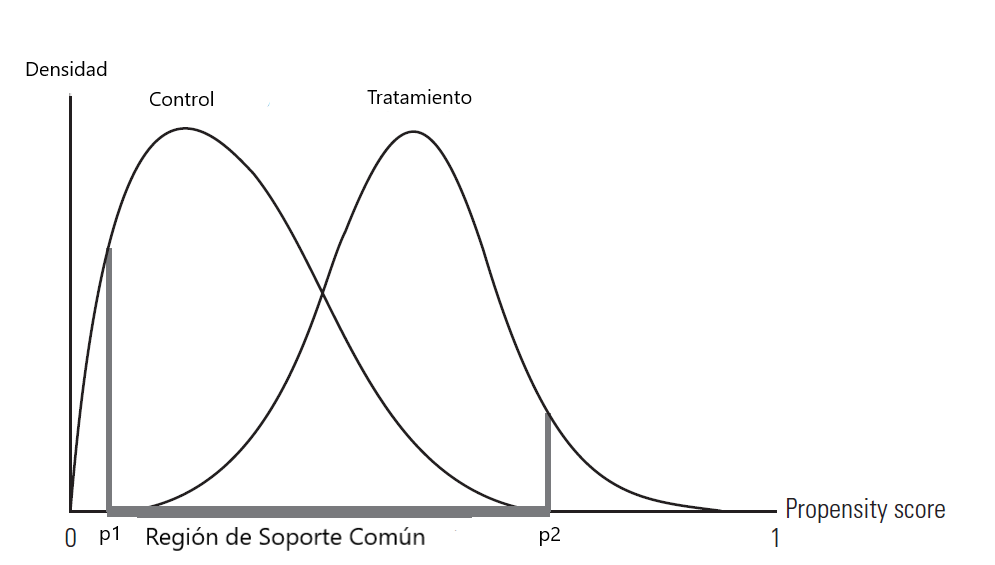
\includegraphics[width=6.7cm, height=6.7cm, keepaspectratio]{Figuras/restriccion-soporte-comun-psm.png}
    \end{figure} 
    \end{center}
    %%\pause
    \smallspace
    \item \textcolor{blue}{Implicación}: los efectos causales sólo son válidos para las unidades que pertenecen al \textbf{soporte común}.
\end{itemize}
\end{frame}


\begin{frame}{Resumiendo: pasos para aplicar PSM}
\begin{itemize}
    \item El teorema del \textcolor{blue}{propensity score} sugiere un procedimiento en cuatro pasos:
    \smallspace
    \begin{enumerate}
        \item \textbf{Estimar} el \textcolor{blue}{propensity score} \(\hat{p}_i\) para cada unidad (e.g., \textit{logit}, \textit{probit}). %%\pause
        \smallspace
        \item \textbf{Restringir} la muestra a la región de \textcolor{blue}{soporte común}: \{i: \(\hat{p}_i \in \mathcal{S}\)\}. %%\pause
        \smallspace
        \item \textbf{Emparejar} tratados y controles con valores similares de \(\hat{p}_i\). %%\pause
        \smallspace
        \item \textbf{Estimar} el efecto: comparar resultados entre unidades emparejadas y promediar para obtener el \textbf{efecto promedio del tratamiento}.
    \end{enumerate}
\end{itemize}
\end{frame}


%%%%%%%%%%%%%%%%%%%%%%%%%%%%%%%%%%%%%%%%%%%%%%%%%%%%%%%%%%%%%%
%%%%%%%%%%%%%%%%%%%%%%%%%%%%%%%%%%%%%%%%%%%%%%%%%%%%%%%%%%%%%%
\subsection{- Algoritmos de emparejamiento}

\begin{frame}{Algoritmos de emparejamiento: fórmula general}
\begin{itemize}
    \item \textcolor{red}{\textbf{Estimando}} (e.g., ATT en soporte común):
    \vspace{-0.4em}
    \begin{align*}
        \begin{split}
        \textcolor{brown}{\tau_{ATT}} 
        &= \EX\left[\EX[Y_i \mid D_i=1, p_i] - \EX[Y_i \mid D_i=0, p_i]\Big| D_i=1, p_i \in \mathcal{S} \right] \\
        &= \EX\left[\brown{\tau(p_i)}\Big| D_i=1, p_i \in \mathcal{S} \right] \quad \text{donde} \quad p_i \equiv \Pr[D_i=1 \mid \XB_i].
                \end{split}
    \end{align*}
    %%\pause
    \item \textcolor{red}{\textbf{Estimador}}: con una muestra de \(N_1\) tratados en el \textcolor{blue}{soporte común},
    \vspace{-0.7em}
    \[
        \textcolor{brown}{\hat{\tau}_{ATT}} 
        = \frac{1}{N_1}\sum_{\{i: D_i=1,\, \hat{p}_i \in \mathcal{S}\}} 
        \left(\, Y_i - \textcolor{red}{\sum_{\{j: D_j=0,\, \hat{p}_j \in \mathcal{S}\}} 
        \omega(i,j) \, Y_j} \right),
    \]
    %%\pause
    donde:
    \begin{itemize}
        \item \(\omega(i,j)\): peso asignado al control \(j\) al construir el contrafactual de la unidad tratada \(i\), con \(\sum_{\{j: D_j=0,\, \hat{p}_j \in \mathcal{S}\}} \omega(i,j) = 1\) para cada \(i\).
    \end{itemize}
\end{itemize}
\end{frame}


\begin{frame}{Algoritmos de emparejamiento: Vecino más cercano}
\begin{itemize}
	\item Cada unidad tratada $i$ se empareja con la unidad de control $j$ cuyo \textbf{propensity score estimado} sea el más cercano al de $i$:
    \begin{align*}
        j(i)=\argmin_{\{k: D_k=0,\; \hat{p}_k \in \mathcal{S}\}} |\hat{p}_i-\hat{p}_k|, 
        \qquad
        \omega(i,j)=\mathbf{1}\{j=j(i)\}.
    \end{align*}
    En este caso, $\omega(i,j)$ toma el valor de uno para el vecino más cercano y cero de lo contrario. 
    \vspace{0.5em}
    %%\pause
    \item En la práctica, nada garantiza que el \textcolor{blue}{vecino más cercano} sea efectivamente ``cercano''. Es fundamental verificar el \textcolor{blue}{balance} en las covariables $\XB$ entre los grupos de tratamiento y control después del emparejamiento.
\end{itemize}
\end{frame}


\begin{frame}{Vecino más cercano: Algunas consideraciones}
\begin{enumerate}
    \item \textbf{Con reemplazo:} varias unidades tratadas pueden ser emparejadas a la misma unidad en el grupo de control.
    \smallspace
    %%\pause
    \item \textbf{Sin reemplazo:} si la unidad en el grupo de control fue emparejada, no se usa más $\implies$ ¡El orden del emparejamiento importa!
\end{enumerate} 
    %%\pause
\begin{itemize}
    \item Una extensión natural es usar los \textbf{$M$ vecinos más cercanos}, asignando un peso respectivo $\frac{1}{M}$ a cada uno. 
\end{itemize}
\end{frame}


\begin{frame}{Algoritmos de emparejamiento: Distancia máxima}
\begin{itemize}
    \item \textcolor{blue}{Distancia máxima (radio):} cada unidad tratada $i$ se empareja con las unidades de control cuyo \textbf{propensity score} esté a una distancia máxima $q$. Definimos
    \begin{align*}
    L(i,j)=\mathbf{1}\{|\hat{p}_i-\hat{p}_j| \leq q\},
    \end{align*}
    y asignamos el peso 
    \begin{align*}
        \omega(i,j) = 
        \begin{cases}
            \frac{1}{\sum_{\{ k: D_k = 0, \hat{p}_k \in \mathcal{S} \} } L(i,k)} \;\; &\text{si} \;\; L(i,j) = 1 \\
            0 \;\; &\text{si} \;\; L(i,j) = 0.
        \end{cases}
    \end{align*}
    Si ningún control está a distancia \(q\) de \(i\), la unidad tratada se descarta (cambia el estimando).
    %%\pause
    \item En la versión \textcolor{blue}{caliper} de distancia máxima, se usan únicamente los $M$ vecinos más cercanos, condicional a estar a una distancia máxima $q$.
\end{itemize}
\end{frame}


\begin{frame}{Algoritmos de emparejamiento: Kernel}
\begin{itemize}
    \item \textcolor{blue}{Emparejamiento usando función de Kernel:} Asigna mayor peso a las unidades de control más \textbf{cercanas} y menor peso a las más \textbf{lejanas}, según la distancia en el \textbf{propensity score estimado}.
    %%\pause
    \smallspace
    \item El contrafactual predicho para cada unidad $i$ es:
    \smallspace
    \begin{align*}
    \textcolor{red}{\hat{Y}_i(0)} = \frac{\sum_{\{j: D_j=0, \hat{p}_j \in \mathcal{S}\}} K\left(\frac{\hat{p}_i-\hat{p}_j}{h}\right)Y_j}{\sum_{\{j: D_j=0, \hat{p}_j \in \mathcal{S}\}} K\left(\frac{\hat{p}_i-\hat{p}_j}{h}\right)},
    \end{align*} 
    donde $K(\cdot)$ es la \textbf{función Kernel} y $h$ es el \textcolor{blue}{ancho de banda}. 
    %%\pause
    \smallspace
    \item \textcolor{blue}{Estimador}:
    \begin{equation*}
    \textcolor{brown}{\hat{\tau}_{ATT}} = \frac{1}{N_{1}}\sum_{\{i: D_i=1, \hat{p}_i \in \mathcal{S} \}} \left(Y_i - \textcolor{red}{\hat{Y}_i(0)}\right).
    \end{equation*}
\end{itemize}
\end{frame}


\begin{frame}{Funciones de Kernel}
\begin{center}	
\begin{figure}        
    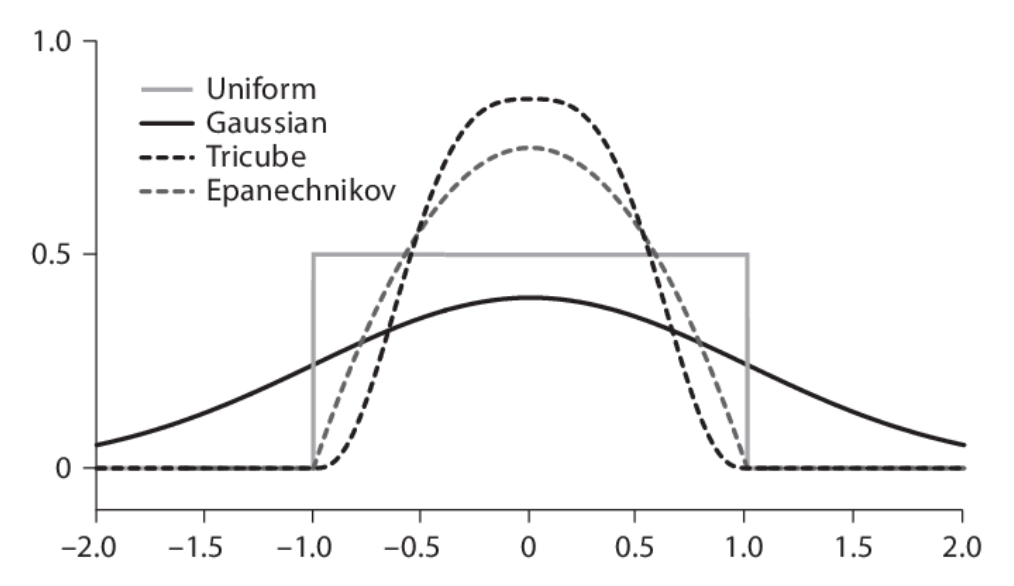
\includegraphics[width=9cm, height=9cm, keepaspectratio]{Figuras/matching-funciones-kernel.png}
\end{figure} 
\end{center}
%%\pause
Por ejemplo, si el Kernel es \textbf{Gaussiano}, los pesos decrecen siguiendo la distribución normal. 
\end{frame}


\begin{frame}{Errores estándar en PSM}
\begin{itemize}
    \item En PSM, los errores estándar deben reflejar tres fuentes de variación: 
    \vspace{-0.0em}
    \begin{enumerate}
        \item[1)] \textbf{Estimación} del propensity score \(\hat{p}_i\).
        \item[2)] \textbf{Restricción} al soporte común.
        \item[3)] \textbf{Algoritmo} de emparejamiento.
    \end{enumerate}
    %%\pause
    \vspace{0.5em}
    El uso de \textcolor{blue}{bootstrapping} \citep{efron1979} es frecuente, pero \textbf{puede ser inconsistente} \citep{abadie2008}.
    %%\pause
    \vspace{1.0em}
    \item \textbf{Alternativas:}
    \begin{itemize}
        \item[-] Usar fórmulas \textbf{analíticas de varianza} para matching \citep{Abadie2006, abadie2016}.
        \item[-] En métodos ``suaves'' (kernel, radio): estimar varianzas con bootstrap, \textbf{re-estimando} \(\hat{p}_i\) y rehaciendo \textit{trimming} en cada réplica.
    \end{itemize}
\end{itemize}
\end{frame}


%%%%%%%%%%%%%%%%%%%%%%%%%%%%%%%%%%%%%%%%%%%%%%%%%%%%%%%%%%%%%%%%%%%%%
%%%%%%%%%%%%%%%%%%%%%%%%%%%%%%%%%%%%%%%%%%%%%%%%%%%%%%%%%%%%%%%%%%%%%
\section{Modelo de regresión lineal}

\begin{frame}{Aproximación a la CEF}
\begin{itemize}
    \item Suponga que, en ausencia de tratamiento, \textbf{modelamos}
    \vspace{-0.5em}
    \begin{align*}
        \EX[Y_i(0) | \XB_i] = \XB_i' \betaB.
    \end{align*}
    %%\pause
    Es una aproximación (proyección lineal), no sabemos la CEF ``real'':
    \smallspace
    \begin{enumerate}
        \item Imponemos una forma funcional que nos puede llevar a \textbf{errores de especificación}. %%\pause
        \smallspace
        \item Si los soportes de \(\XB\) difieren entre tratados y controles, \(\XB_i'\betaB\) puede \textbf{extrapolar}. 
    \end{enumerate}  
    %%\pause
    \vspace{1.0em}
    \item Bajo \textcolor{blue}{independencia condicional} \(Y_i(0),Y_i(1) \indep D_i \mid \XB_i\):
    {\fontvid
    \begin{align*}
        \begin{split}
            Y_i = Y_i(0) + \Big(Y_i(1) - Y_i(0)\Big) D_i \implies \EX [Y_i | \XB_i, D_i] &= \brown{\tau(\XB_i)} D_i + \EX[Y_i(0) | \XB_i] \\
            &\approx \brown{\tau(\XB_i)} D_i + \XB'_i \betaB.
        \end{split}        
    \end{align*}
    }
    donde \(\brown{\tau(\XB_i)} \equiv \EX[Y_i(1) - Y_i(0) | \XB_i]\) son los \textbf{CATE}.
\end{itemize}
\end{frame}


\begin{frame}{El modelo de regresión lineal}
\begin{itemize}
    \item Considere el modelo de regresión:
    \begin{align}\label{REG-LINEAL}
        Y_i= \brown{\tau}D_i + \XB_i'\betaB + e_i.
    \end{align}
    ¿Cómo se relacionan \(\EX[\brown{\tau(\XB_i)}] \) y \(\brown{\tau}\)? ¿Qué está estimando MCO?
    %%\pause
    \vspace{1em}
  \item Por el teorema de \textbf{Frisch–Waugh–Lovell} (FWL), estimar \eqref{REG-LINEAL} por MCO es equivalente a estimar
  \begin{align*}
      \tilde{Y}_i &= \brown{\tau} \tilde{D}_i + \eta_i,
  \end{align*}
  donde $\tilde Y_i$ y $\tilde D_i$ son los \textbf{residuales de la proyección lineal} de \(Y_i\) y \(D_i\) en \(\XB_i\), respectivamente.
\end{itemize}
\end{frame}


\begin{frame}{¿Qué estima MCO en el modelo de regresión lineal?}\label{DIAP:MCO}
\begin{itemize}
    \item Bajo \textcolor{blue}{ignorabilidad fuerte}, si \(p_i\) es \textbf{lineal en los controles incluidos} (p. ej., una especificación saturada), se puede \hyperlink{Demostracion-MCO}{{\beamerreturnbutton{demostrar}}} que:
    \begin{align*}  
          \plim \brown{\hat\tau_{mco}}
     = \frac{\EX \big[ \brown{\tau(\XB_i)} \omega(\XB_i)\big]}
            {\EX\!\big[\omega(\XB_i)\,\big]} \neq \EX[\brown{\tau(\XB_i)}] \;\; \text{(en general)},
    \end{align*}
    donde \(\omega(\XB_i) \equiv \EX[\tilde D_i^{2} \mid \XB_i] = p_i(1-p_i)\).
    \vspace{1em}
    %%\pause
    \item MCO estima un promedio ponderado de los \textbf{CATE}, con pesos proporcionales a la varianza condicional del tratamiento: \textcolor{blue}{actúa como un estimador de \emph{matching} con pesos específicos.} %%\pause
    \vspace{1em}
    \item Si los efectos son \textbf{homogéneos}: \(\brown{\tau(\XB_i)}= \brown{\tau} \; \forall \; \XB_i\), se cumple que \(\plim \brown{\hat\tau_{mco}} = \EX[\brown{\tau(\XB_i)}] = \brown{\tau}.\) De lo contrario, el efecto estimado puede diferir de los obtenidos con estimadores de \emph{matching}.
\end{itemize}    
\end{frame}


\begin{frame}{Extrapolación si la CEF no es lineal}
\begin{itemize}
  \item \textcolor{blue}{Error de especificación}: si \(p_i\) no es lineal en los controles incluidos, la fórmula anterior \textbf{no está garantizada} y puede haber sesgo por una forma funcional incorrecta. %%\pause
  \vspace{1em}
  \item \textcolor{blue}{Problema de extrapolación}: con \textbf{pobre \textit{overlap}} entre tratados y controles, el contrafactual de algunos tratados se construye usando observaciones ``lejanas'' en el espacio de covariables. %%\pause
  \vspace{1em}
  \item \textbf{Consecuencia}: aun bajo los supuestos anteriores, \(\brown{\hat\tau_{mco}}\) puede ser \textbf{inconsistente} para el ATE (o el ATT) por sus pesos sobre los CATE. El poco \textit{overlap} puede reducir la precisión.
\end{itemize}
\end{frame}


\begin{frame}{Forma funcional y extrapolación en MCO: una simulación}
% Simulación hecha una vez en numpy (documentada aquí para reproducirla):
% DGP: Y_i(0)=Y_i(1)=X_i^2+eps_i, eps~N(0,1); por muestra, 50 controles con X~U[0,2]
% y 50 tratados con X~U[3,4] (p(x) es 0 o 1: sin soporte común). MCO de Y en (1,D,X).
% plim tau_mco = 3.50 (alpha=-1.67, beta=3.00). Panel izq.: seed 1 -> tau_hat=3.513,
% alpha=-1.838, beta=3.039 (rectas graficadas). Panel der.: 5000 réplicas por tamaño;
% N=100: media 3.47, sd 0.72; N=1000: media 3.50, sd 0.22 (histogramas en densidad).
% Ojo: sin \begingroup, el grupo {\footnotesize...} sería tragado como subtítulo del frame.
\begin{itemize}
    \item Se cumple \textcolor{blue}{independencia condicional}, pero \textbf{no hay soporte común}.


\vspace{1.0em}
\begin{columns}[T,onlytextwidth]
\begin{column}{0.49\textwidth}
\centering
{\small \textbf{Una muestra} (\(N=100\))}\\[0.05em]
{\scriptsize \textcolor{blue}{\(\bullet\)} Controles\quad
\textcolor{brown}{\(\blacktriangle\)} Tratados\quad
\tikz[baseline=-0.5ex]{\draw[gray,thick] (0,0)--(0.35,0);} CEF verdadera}
\begin{tikzpicture}
\begin{axis}[
    width=\linewidth, height=3.9cm,
    xmin=-0.2, xmax=5.0, ymin=-2, ymax=20,
    xlabel={\(X_i\)}, ylabel={\(Y_i\)},
    xtick={0,2,4}, ytick={0,8,16},
    tick label style={font=\footnotesize}, label style={font=\small},
    axis lines=left, clip=false,
]
    \path[fill=blue!6] (axis cs:2,-2) rectangle (axis cs:4.9,19.6);
    \node[font=\scriptsize, anchor=north] at (axis cs:3.45,19.4)
        {Sin controles};
    \addplot[gray, thick, domain=0:4, samples=81] {x^2};
    \addplot[blue, thick, domain=0:2] {-1.838+3.039*x};
    \addplot[blue, thick, dashed, domain=2:4.35] {-1.838+3.039*x};
    \addplot[brown, thick, domain=2.9:4.35] {1.675+3.039*x};
    \addplot[only marks, blue, mark=*, mark size=1.1pt] coordinates {
        (1.024,1.381) (1.901,2.962) (0.288,0.946) (1.897,3.474) (0.624,1.058)
        (0.847,1.936) (1.655,3.123) (0.818,-0.206) (1.099,-0.306) (0.055,1.756)
        (1.507,2.160) (1.076,0.470) (0.659,0.579) (1.577,2.295) (0.606,1.220)
        (0.907,0.857) (0.268,0.086) (0.806,-0.065) (0.407,0.635) (0.525,-0.759)
        (1.501,2.918) (0.561,1.838) (0.970,-0.583) (1.961,1.381) (1.923,4.316)
        (1.450,4.649) (1.082,0.171) (0.554,-0.944) (0.321,0.692) (1.940,2.922)
        (1.032,0.559) (0.232,-0.294) (1.247,2.087) (1.553,2.008) (1.226,1.781)
        (1.835,3.189) (0.079,-0.838) (1.057,0.798) (0.919,-0.106) (0.125,0.022)
        (1.283,0.521) (1.705,1.815) (1.186,2.863) (0.520,0.217) (1.680,2.768)
        (1.019,1.550) (1.022,0.623) (1.506,2.040) (0.296,0.513) (1.639,2.970)
    };
    \addplot[only marks, brown, mark=triangle*, mark size=1.5pt] coordinates {
        (3.683,12.407) (3.787,15.175) (3.192,9.596) (3.802,13.402) (3.191,9.284)
        (3.082,9.105) (3.855,16.490) (3.861,13.734) (3.877,15.188) (3.472,9.916)
        (3.274,10.718) (3.007,9.942) (3.646,13.055) (3.720,13.208) (3.836,14.943)
        (3.282,11.471) (3.215,11.001) (3.639,15.217) (3.805,14.688) (3.964,15.118)
        (3.151,9.800) (3.482,12.053) (3.895,15.278) (3.423,11.685) (3.590,13.058)
        (3.024,7.477) (3.673,14.324) (3.919,14.785) (3.827,13.471) (3.886,15.735)
        (3.660,14.716) (3.246,11.027) (3.769,14.363) (3.212,9.383) (3.831,17.550)
        (3.063,10.260) (3.825,13.495) (3.165,9.234) (3.375,11.479) (3.317,9.446)
        (3.691,13.795) (3.179,9.644) (3.396,12.761) (3.006,9.997) (3.262,7.933)
        (3.421,11.746) (3.106,8.029) (3.633,14.309) (3.380,11.595) (3.725,14.426)
    };
    \draw[<->, brown, thick] (axis cs:4.15,10.774) -- (axis cs:4.15,14.287)
        node[midway, right, font=\footnotesize] {\(\brown{\hat\tau_{mco}}\)};
\end{axis}
\end{tikzpicture}
\par\smallskip
\raggedright\footnotesize
MCO impone rectas paralelas (\textbf{forma funcional}) y usa la recta azul donde no hay controles (\textbf{extrapolación}): \(\brown{\hat\tau_{mco}}\approx 3.5\).
\end{column}
\begin{column}{0.49\textwidth}
\centering
{\small \textbf{5000 muestras}: distribución de \(\brown{\hat\tau_{mco}}\)}\\[0.05em]
{\scriptsize \textcolor{gray!80}{\(\blacksquare\)} \(N=100\)\quad
\textcolor{blue!70}{\(\blacksquare\)} \(N=1000\)\quad
\tikz[baseline=-0.5ex]{\draw[red,very thick] (0,0)--(0.35,0);} \(\tau\) verdadero}
\begin{tikzpicture}
\begin{axis}[
    width=\linewidth, height=3.9cm,
    xmin=-0.9, xmax=6.6, ymin=0, ymax=2.15,
    xlabel={\(\brown{\hat\tau_{mco}}\)}, ylabel={Densidad},
    xtick={0,3.5}, ytick={0,1,2},
    tick label style={font=\footnotesize}, label style={font=\small},
    axis lines=left, clip=false,
]
    \addplot[ybar interval, fill=gray!35, draw=gray!70, very thin] coordinates {
        (1.20,0.007) (1.35,0.020) (1.50,0.016) (1.65,0.021) (1.80,0.052)
        (1.95,0.061) (2.10,0.120) (2.25,0.151) (2.40,0.225) (2.55,0.283)
        (2.70,0.325) (2.85,0.407) (3.00,0.469) (3.15,0.507) (3.30,0.541)
        (3.45,0.533) (3.60,0.552) (3.75,0.543) (3.90,0.465) (4.05,0.337)
        (4.20,0.311) (4.35,0.224) (4.50,0.147) (4.65,0.147) (4.80,0.071)
        (4.95,0.060) (5.10,0.029) (5.25,0.012) (5.40,0.011) (5.55,0.007)
        (5.70,0.004) (5.85,0.003) (6.00,0.001) (6.15,0)
    };
    \addplot[ybar interval, fill=blue!60, draw=blue!65!black, very thin,
             fill opacity=0.6] coordinates {
        (2.70,0.016) (2.85,0.076) (3.00,0.305) (3.15,0.861) (3.30,1.488)
        (3.45,1.780) (3.60,1.316) (3.75,0.620) (3.90,0.176) (4.05,0.023)
        (4.20,0.005) (4.35,0)
    };
    \draw[red, very thick] (axis cs:0,0) -- (axis cs:0,1.9)
        node[above right, font=\footnotesize, red, inner sep=1.5pt] {\(\tau=0\)};
\end{axis}
\end{tikzpicture}
\par\smallskip
\raggedright\footnotesize
El sesgo es \textbf{sistemático}: \(\brown{\hat\tau_{mco}}\) se concentra alrededor de \(3.5\), no de \(\tau=0\). Más datos \(\Rightarrow\) más precisión, \textbf{no} menos sesgo.
\end{column}
\end{columns}
\end{itemize}
\end{frame}


\begin{frame}
\begin{tcolorbox}[colback=white, title=\citet{Angrist2008}, arc=0mm,boxrule=0.5pt, breakable]
``\textit{\textcolor{blue}{We believe regression should be the starting point for most empirical projects.} This is not a theorem; undoubtedly, there are circumstances where propensity  score matching provides more reliable estimates of average causal effects. \textcolor{blue}{The first reason we don’t find ourselves on the propensity-score bandwagon is practical: there are many details to be filled in when implementing propensity-score matching} – such as how to model the score and how to do inference – these details are not yet standardized. Different researchers might therefore reach very different conclusions, even when using the same data and covariates.}''
\end{tcolorbox}
\end{frame}


\begin{frame}
\begin{tcolorbox}[colback=white, title=\citet{Imbens2015a}, arc=0mm,boxrule=0.5pt, breakable]
``\textit{Researchers continue to use ordinary linear regression methods with an indicator for the treatment and covariates entering additively and linearly. However, such simple methods do not always work well... \textcolor{blue}{the simple ordinary least squares estimator, which ultimately relies on the same fundamental unconfoundedness assumption as matching and propensity score estimators, but combines that assumption with strong functional form restrictions, is likely to be inadequate for estimating average treatment effects.}}''
\end{tcolorbox}
\end{frame}


%%%%%%%%%%%%%%%%%%%%%%%%%%%%%%%%%%%%%%%%%%%%%%%%%%%%%%%%%%%%%%%%%%%%%
%%%%%%%%%%%%%%%%%%%%%%%%%%%%%%%%%%%%%%%%%%%%%%%%%%%%%%%%%%%%%%%%%%%%%
\section{Inverse Probability Weighting (IPW)}

\begin{frame}{Inverse Probability Weighting (IPW)}\label{DIAP:DEMOS}
\begin{itemize}
    \item Suponga que se cumple \textcolor{blue}{ignorabilidad fuerte}:
    \vspace{-0.1em}
    \begin{align*}
        Y_i(0),Y_i(1) \indep D_i \mid \XB_i,\quad p_i \equiv \Pr[D_i=1\mid \XB_i] \in (0,1),
    \end{align*} 
    entonces se cumple la siguiente \textbf{identidad} \citep{horvitz1952}:
    \vspace{-0.85em}
    \begin{align*}
        \EX \Big[\frac{D_i Y_i}{p_i}\Big]=\EX[Y_i(1)], 
        \quad
        \EX \Big[\frac{(1-D_i) Y_i}{1-p_i}\Big]=\EX[Y_i(0)].
    \end{align*}    
    \hyperlink{Demostracion-IPW}{{\beamerreturnbutton{Demostración}}}%%\pause \hspace{0.5em} En consecuencia,    
    \vspace{-1.2em} 
    \begin{align*}
        \brown{\tau_{ATE}} = \EX \Big[\frac{D_i Y_i}{p_i} - \frac{(1-D_i) Y_i}{1-p_i}\Big].      
    \end{align*}
    %%\pause
    \item Esto motiva el \textbf{estimador IPW} en la práctica:
    \vspace{-0.6em}
    \begin{align*}
    \brown{\hat\tau_{\text{IPW}}}
    = \frac{1}{N}\sum_{i}
      \left(\frac{D_i Y_i}{\hat p_i}
      - \frac{(1-D_i) Y_i}{1-\hat p_i}\right). 
    \end{align*}
\end{itemize}
\end{frame}


\begin{frame}{IPW normalizado (Hájek)}
\begin{itemize}
  \item El estimador IPW de \citet{horvitz1952} puede tener alta varianza porque los pesos
  \begin{align*}
      \omega_i(1) = \frac{D_i}{\hat p_i}, \quad \omega_i(0) = \frac{1-D_i}{1-\hat p_i},
  \end{align*}
  no necesariamente suman \(N\) en la muestra (su valor esperado). %%\pause
  \vspace{0.5em}
  \item \textcolor{blue}{IPW de Hájek (normalizado)}: reescala los pesos dentro de cada grupo,
  \begin{align*}     
    \brown{\hat\tau_{\text{IPW}}^{H}} 
    = 
    \frac{\sum_{i} \frac{D_i Y_i}{\hat p_i}}
                      {\sum_{i} \frac{D_i}{\hat p_i}}
    -
    \frac{\sum_{i} \frac{(1-D_i) Y_i}{1-\hat p_i}}
                      {\sum_{i} \frac{(1-D_i)}{1-\hat p_i}},
  \end{align*}
  donde \(\frac{1}{N}\sum_i \frac{D_i}{\hat p_i} \;\xrightarrow{p} 1\) y \(\frac{1}{N}\sum_i \frac{1-D_i}{1 -\hat p_i} \;\xrightarrow{p} 1\). Este estimador es \textbf{consistente} y suele tener menor varianza. También hace que el estimador se interprete como una media ponderada usual.
\end{itemize}
\end{frame}


\begin{frame}{IPW: intuición no técnica}
\begin{itemize}
  \item Si tratados y controles difieren en sus covariables \(\XB\), un \textit{promedio directo} compara \textcolor{blue}{manzanas con peras}. %%\pause
  \vspace{1em}
  \item El \textbf{IPW repondera} las observaciones según su \textit{propensity score}:
  \smallspace
  \begin{itemize}
    \item Más peso a las unidades \textcolor{blue}{raras} (con baja probabilidad de estar en su grupo).
    \item Menos peso a las unidades \textcolor{blue}{comunes}. %%\pause
  \end{itemize}
  \vspace{1em}
  De esta forma, la muestra ponderada queda \textbf{balanceada}: tratados y controles terminan con distribuciones comparables de \(\XB\). %%\pause
  \vspace{1em}
  \item El promedio ponderado elimina el sesgo de composición y aproxima el \textbf{efecto causal promedio}.
\end{itemize}
\end{frame}


\begin{frame}{IPW balancea el propensity score}
% Simulación hecha una vez en numpy (seed 1, N=5000), compartida con la diapositiva
% siguiente: X1=(chi2(4)-4)/sqrt(8) (asimétrica, media 0, sd 1); X2=0.4*X1+sqrt(0.84)*N(0,1);
% p(X)=Lambda(0.9*X1+0.6*X2); D~Bernoulli(p) (48% tratados). p_hat por logit (IRLS);
% pesos ATE tipo Hájek: D/p_hat y (1-D)/(1-p_hat), normalizados dentro de cada grupo.
% Curvas: KDE gaussiano (h=0.05) de p_hat, ponderado por los pesos indicados.
% Overlap se cumple: max p_hat entre controles = 0.986; peso máximo de un control = 1.5% del total.
\begingroup\centering\scriptsize
\tikz[baseline=-0.5ex]{\draw[blue,thick] (0,0)--(0.35,0);} Controles\quad
\tikz[baseline=-0.5ex]{\draw[brown,thick] (0,0)--(0.35,0);} Tratados\quad
\tikz[baseline=-0.5ex]{\draw[gray,thick,densely dashed] (0,0)--(0.35,0);} Población\par
\endgroup
\begin{columns}[T,onlytextwidth]
\begin{column}{0.49\textwidth}
\centering
{\small \textbf{Sin ajuste}}
\begin{tikzpicture}
\begin{axis}[
    width=\linewidth, height=3.8cm,
    xmin=0, xmax=1, ymin=0, ymax=2.5,
    xlabel={\(\hat p_i\)}, ylabel={Densidad},
    xtick={0,0.5,1}, ytick={0,1,2},
    tick label style={font=\footnotesize}, label style={font=\small},
    axis lines=left,
]
    \addplot[gray, thick, densely dashed] coordinates {
        (0.00,0.034) (0.02,0.071) (0.04,0.132) (0.06,0.224) (0.08,0.350)
        (0.10,0.506) (0.12,0.684) (0.14,0.872) (0.16,1.054) (0.18,1.217)
        (0.20,1.353) (0.22,1.458) (0.24,1.536) (0.26,1.588) (0.28,1.618)
        (0.30,1.630) (0.32,1.628) (0.34,1.614) (0.36,1.592) (0.38,1.561)
        (0.40,1.522) (0.42,1.474) (0.44,1.419) (0.46,1.361) (0.48,1.306)
        (0.50,1.259) (0.52,1.219) (0.54,1.185) (0.56,1.152) (0.58,1.117)
        (0.60,1.079) (0.62,1.042) (0.64,1.007) (0.66,0.975) (0.68,0.943)
        (0.70,0.911) (0.72,0.880) (0.74,0.851) (0.76,0.825) (0.78,0.800)
        (0.80,0.777) (0.82,0.753) (0.84,0.729) (0.86,0.705) (0.88,0.679)
        (0.90,0.647) (0.92,0.603) (0.94,0.542) (0.96,0.462) (0.98,0.369)
        (1.00,0.270)
    };
    \addplot[blue, thick] coordinates {
        (0.00,0.058) (0.02,0.120) (0.04,0.222) (0.06,0.375) (0.08,0.581)
        (0.10,0.834) (0.12,1.114) (0.14,1.397) (0.16,1.658) (0.18,1.875)
        (0.20,2.038) (0.22,2.148) (0.24,2.210) (0.26,2.232) (0.28,2.221)
        (0.30,2.182) (0.32,2.124) (0.34,2.051) (0.36,1.970) (0.38,1.882)
        (0.40,1.790) (0.42,1.692) (0.44,1.588) (0.46,1.479) (0.48,1.371)
        (0.50,1.269) (0.52,1.177) (0.54,1.094) (0.56,1.016) (0.58,0.939)
        (0.60,0.863) (0.62,0.790) (0.64,0.721) (0.66,0.656) (0.68,0.594)
        (0.70,0.533) (0.72,0.476) (0.74,0.422) (0.76,0.374) (0.78,0.332)
        (0.80,0.293) (0.82,0.256) (0.84,0.218) (0.86,0.181) (0.88,0.145)
        (0.90,0.113) (0.92,0.086) (0.94,0.065) (0.96,0.048) (0.98,0.034)
        (1.00,0.023)
    };
    \addplot[brown, thick] coordinates {
        (0.00,0.008) (0.02,0.018) (0.04,0.035) (0.06,0.062) (0.08,0.101)
        (0.10,0.154) (0.12,0.223) (0.14,0.307) (0.16,0.404) (0.18,0.510)
        (0.20,0.616) (0.22,0.717) (0.24,0.811) (0.26,0.895) (0.28,0.970)
        (0.30,1.037) (0.32,1.095) (0.34,1.145) (0.36,1.186) (0.38,1.216)
        (0.40,1.234) (0.42,1.239) (0.44,1.237) (0.46,1.234) (0.48,1.237)
        (0.50,1.248) (0.52,1.265) (0.54,1.284) (0.56,1.299) (0.58,1.307)
        (0.60,1.311) (0.62,1.313) (0.64,1.315) (0.66,1.318) (0.68,1.319)
        (0.70,1.317) (0.72,1.315) (0.74,1.312) (0.76,1.309) (0.78,1.304)
        (0.80,1.297) (0.82,1.288) (0.84,1.278) (0.86,1.269) (0.88,1.254)
        (0.90,1.222) (0.92,1.159) (0.94,1.055) (0.96,0.908) (0.98,0.728)
        (1.00,0.537)
    };
\end{axis}
\end{tikzpicture}
\end{column}
\begin{column}{0.49\textwidth}
\centering
{\small \textbf{Con ajuste por IPW}}
\begin{tikzpicture}
\begin{axis}[
    width=\linewidth, height=3.8cm,
    xmin=0, xmax=1, ymin=0, ymax=2.5,
    xlabel={\(\hat p_i\)}, ylabel={Densidad},
    xtick={0,0.5,1}, ytick={0,1,2},
    tick label style={font=\footnotesize}, label style={font=\small},
    axis lines=left,
]
    \addplot[gray, thick, densely dashed] coordinates {
        (0.00,0.034) (0.02,0.071) (0.04,0.132) (0.06,0.224) (0.08,0.350)
        (0.10,0.506) (0.12,0.684) (0.14,0.872) (0.16,1.054) (0.18,1.217)
        (0.20,1.353) (0.22,1.458) (0.24,1.536) (0.26,1.588) (0.28,1.618)
        (0.30,1.630) (0.32,1.628) (0.34,1.614) (0.36,1.592) (0.38,1.561)
        (0.40,1.522) (0.42,1.474) (0.44,1.419) (0.46,1.361) (0.48,1.306)
        (0.50,1.259) (0.52,1.219) (0.54,1.185) (0.56,1.152) (0.58,1.117)
        (0.60,1.079) (0.62,1.042) (0.64,1.007) (0.66,0.975) (0.68,0.943)
        (0.70,0.911) (0.72,0.880) (0.74,0.851) (0.76,0.825) (0.78,0.800)
        (0.80,0.777) (0.82,0.753) (0.84,0.729) (0.86,0.705) (0.88,0.679)
        (0.90,0.647) (0.92,0.603) (0.94,0.542) (0.96,0.462) (0.98,0.369)
        (1.00,0.270)
    };
    \addplot[blue, thick] coordinates {
        (0.00,0.034) (0.02,0.070) (0.04,0.130) (0.06,0.222) (0.08,0.348)
        (0.10,0.505) (0.12,0.684) (0.14,0.871) (0.16,1.051) (0.18,1.210)
        (0.20,1.342) (0.22,1.445) (0.24,1.521) (0.26,1.574) (0.28,1.606)
        (0.30,1.621) (0.32,1.622) (0.34,1.612) (0.36,1.595) (0.38,1.572)
        (0.40,1.543) (0.42,1.507) (0.44,1.462) (0.46,1.411) (0.48,1.357)
        (0.50,1.307) (0.52,1.263) (0.54,1.225) (0.56,1.189) (0.58,1.150)
        (0.60,1.108) (0.62,1.066) (0.64,1.026) (0.66,0.988) (0.68,0.948)
        (0.70,0.906) (0.72,0.864) (0.74,0.827) (0.76,0.795) (0.78,0.769)
        (0.80,0.744) (0.82,0.714) (0.84,0.676) (0.86,0.631) (0.88,0.586)
        (0.90,0.552) (0.92,0.528) (0.94,0.507) (0.96,0.471) (0.98,0.408)
        (1.00,0.321)
    };
    \addplot[brown, thick] coordinates {
        (0.00,0.039) (0.02,0.083) (0.04,0.154) (0.06,0.255) (0.08,0.385)
        (0.10,0.537) (0.12,0.707) (0.14,0.887) (0.16,1.070) (0.18,1.243)
        (0.20,1.392) (0.22,1.507) (0.24,1.586) (0.26,1.633) (0.28,1.655)
        (0.30,1.658) (0.32,1.646) (0.34,1.623) (0.36,1.591) (0.38,1.549)
        (0.40,1.496) (0.42,1.433) (0.44,1.366) (0.46,1.302) (0.48,1.247)
        (0.50,1.205) (0.52,1.173) (0.54,1.145) (0.56,1.118) (0.58,1.087)
        (0.60,1.054) (0.62,1.021) (0.64,0.990) (0.66,0.962) (0.68,0.934)
        (0.70,0.907) (0.72,0.880) (0.74,0.854) (0.76,0.829) (0.78,0.805)
        (0.80,0.781) (0.82,0.756) (0.84,0.733) (0.86,0.710) (0.88,0.686)
        (0.90,0.656) (0.92,0.611) (0.94,0.547) (0.96,0.465) (0.98,0.369)
        (1.00,0.269)
    };
\end{axis}
\end{tikzpicture}
\end{column}
\end{columns}
\begin{itemize}
    \item \textbf{Sin ajuste:} las distribuciones de \(\hat p_i\) de tratados y controles son muy distintas.
    \item \textbf{Con IPW:} al ponderar cada grupo por sus pesos, ambas distribuciones se aproximan a la de la \textbf{población}.
\end{itemize}
\end{frame}


\begin{frame}{IPW balancea las covariables}
% Misma simulación de la diapositiva anterior (seed 1, N=5000). SMD con desviación
% estándar combinada del grupo SIN ajustar (convención de cobalt/tebalance):
% SMD sin ajuste:  X1=0.868, X2=0.781, X1^2=0.341, X2^2=0.073, X1*X2=0.220.
% SMD con IPW:     X1=-0.012, X2=-0.005, X1^2=0.004, X2^2=0.009, X1*X2=0.010.
\begingroup\centering\scriptsize
\textcolor{brown}{\(\blacktriangle\)} Sin ajuste\quad
\textcolor{blue}{\(\bullet\)} Con IPW\quad
\tikz[baseline=-0.5ex]{\draw[gray,densely dashed] (0,0)--(0.35,0);} \(|SMD|=0.1\)\par
\endgroup
\begin{center}
\begin{tikzpicture}
\begin{axis}[
    width=9.2cm, height=3.9cm,
    xmin=-0.2, xmax=1.0, ymin=0.4, ymax=5.6,
    xlabel={Diferencia estandarizada de medias (SMD)},
    xtick={0,0.5,1},
    ytick={1,2,3,4,5},
    yticklabels={\(X_1 X_2\),\(X_2^2\),\(X_1^2\),\(X_2\),\(X_1\)},
    tick label style={font=\footnotesize}, label style={font=\small},
    axis lines=left, clip=false,
]
    \draw[gray!60] (axis cs:0,0.4) -- (axis cs:0,5.6);
    \draw[gray, densely dashed] (axis cs:-0.1,0.4) -- (axis cs:-0.1,5.6);
    \draw[gray, densely dashed] (axis cs:0.1,0.4) -- (axis cs:0.1,5.6);
    \draw[gray!60, thin] (axis cs:-0.012,5) -- (axis cs:0.868,5);
    \draw[gray!60, thin] (axis cs:-0.005,4) -- (axis cs:0.781,4);
    \draw[gray!60, thin] (axis cs:0.004,3) -- (axis cs:0.341,3);
    \draw[gray!60, thin] (axis cs:0.009,2) -- (axis cs:0.073,2);
    \draw[gray!60, thin] (axis cs:0.010,1) -- (axis cs:0.220,1);
    \addplot[only marks, brown, mark=triangle*, mark size=2.4pt] coordinates {
        (0.868,5) (0.781,4) (0.341,3) (0.073,2) (0.220,1)
    };
    \addplot[only marks, blue, mark=*, mark size=2.0pt] coordinates {
        (-0.012,5) (-0.005,4) (0.004,3) (0.009,2) (0.010,1)
    };
\end{axis}
\end{tikzpicture}
\end{center}
\vspace{-0.4em}
{\centering\scriptsize
\textbf{Nota:} misma simulación anterior. \(SMD = (\bar{x}_T - \bar{x}_C)/\sqrt{(s_T^2 + s_C^2)/2}\), con desviaciones de la muestra sin ajustar.\par}
\begin{itemize}
    \item El propensity score es un \textbf{balancing score}: igualar su distribución equilibra \textbf{todas} las covariables, incluidas transformaciones e interacciones.
    \item En la práctica: \textbf{reportar el balance} antes y después de ponderar.
\end{itemize}
\end{frame}

%%%%%%%%%%%%%%%%%%%%%%%%%%%%%%%%%%%%%%%%%%%%%%%%%%%%%%%%%%%%%%
%%%%%%%%%%%%%%%%%%%%%%%%%%%%%%%%%%%%%%%%%%%%%%%%%%%%%%%%%%%%%%

\section{Anexo}

\begin{frame}{Demostración: teorema del propensity score (I)}\label{Demostracion-PS}
\begin{itemize}
    \item Como \(D_i\) es \textbf{binaria}, su distribución condicional está determinada por su media. Basta entonces demostrar que
    \[
    \begin{aligned}
    \mathbb{E}[D_i \mid Y_i(0), Y_i(1), p_i]
    &= \Pr[D_i=1 \mid Y_i(0), Y_i(1), p_i] \\
    &= \Pr[D_i=1 \mid p_i] \\
    &= \mathbb{E}[D_i \mid p_i].
    \end{aligned}
    \]
    es decir, que condicional en \(p_i\), la asignación no depende de \(\big(Y_i(0), Y_i(1)\big)\).
    %%\pause
    \vspace{0.5em}
    \item Por la \textbf{ley de expectativas iteradas} (condicionando primero en \(\XB_i\), que determina \(p_i\)):
    \[
        \EX[D_i \mid Y_i(0), Y_i(1), p_i]
        = \EX\big[\EX[D_i \mid Y_i(0), Y_i(1), \XB_i] \big| Y_i(0), Y_i(1), p_i \big].
    \]
\end{itemize}
\end{frame}


\begin{frame}{Demostración: teorema del propensity score (II)}
\begin{itemize}
    \item Bajo \textcolor{blue}{independencia condicional}, \(\fontvid \EX[D_i \mid Y_i(0), Y_i(1), \XB_i] = \EX[D_i \mid \XB_i]\), donde \(\EX[D_i \mid \XB_i] = p_i\). Por consiguiente
    \[
        \EX[D_i \mid Y_i(0), Y_i(1), p_i] = \EX[p_i \mid Y_i(0), Y_i(1), p_i] = p_i.
    \]
    %%\pause
    \item De forma análoga, por la \textbf{ley de expectativas iteradas}:
    \[
        \EX[D_i \mid p_i] = \EX\big[\EX[D_i \mid \XB_i] \mid p_i\big] = \EX[p_i \mid p_i] = p_i.
    \]
    \item Se desprende que
    \[
    \begin{aligned}
    \mathbb{E}[D_i \mid Y_i(0), Y_i(1), p_i]
    = \mathbb{E}[D_i \mid p_i],
    \end{aligned}
    \]    
    %%\pause
    y podemos concluir que \(Y_i(0), Y_i(1) \indep D_i \mid p_i\).
\end{itemize}
\hyperlink{DIAP:PS}{{\beamerreturnbutton{Regresar}}}
\end{frame}


\begin{frame}{Demostración: $\plim \hat\tau_{mco}$ (I)}\label{Demostracion-MCO}
\begin{itemize}
    \item Por \textbf{FWL}, con \(\tilde D_i\) y \(\tilde Y_i\) los residuales de la \textbf{proyección lineal} en \(\XB_i\) (incluida la constante):
    \[
        \plim \brown{\hat\tau_{mco}} = \frac{\EX[\tilde D_i \, \tilde Y_i]}{\EX[\tilde D_i^{\,2}]}.
    \]
    %%\pause
    \item \textbf{Supuesto}: \(p_i \equiv \EX[D_i \mid \XB_i]\) es lineal en \(\XB_i\). Así, \(\tilde D_i = D_i - p_i\) y \(\EX[\tilde D_i \mid \XB_i]=0\).
    %%\pause
    \item Usando resultados potenciales: \(Y_i = Y_i(0) + D_i \tau_i\), donde \(\tau_i \equiv Y_i(1) - Y_i(0)\). Entonces:
    \[
        \EX[\tilde D_i \, Y_i \mid \XB_i]
        = \underbrace{\EX[(D_i - p_i) Y_i(0) \mid \XB_i]}_{\text{Término A}}
        + \underbrace{\EX[(D_i - p_i) D_i \tau_i \mid \XB_i]}_{\text{Término B}}.
    \]
\end{itemize}
\end{frame}


\begin{frame}{Demostración: $\plim \hat\tau_{mco}$ (II)}
\begin{itemize}
    \item \textbf{Término A}: bajo \textcolor{blue}{ignorabilidad}, \(Y_i(0) \indep D_i \mid \XB_i\), por lo que
    \[
        \EX[(D_i - p_i) Y_i(0) \mid \XB_i]
        = \EX[D_i - p_i \mid \XB_i] \, \EX[Y_i(0) \mid \XB_i] = 0.
    \]
    %%\pause
    \item \textbf{Término B}: como \(D_i \in \{0,1\}\), se tiene \(D_i^2 = D_i\), de modo que
    \[
        (D_i - p_i) D_i = (1 - p_i) D_i.
    \]
    Además, bajo \textcolor{blue}{ignorabilidad}, \(\tau_i \indep D_i \mid \XB_i\), luego
    \begin{align*}
        \EX[(1 - p_i) D_i \tau_i \mid \XB_i]
        &= (1 - p_i) \, \EX[D_i \mid \XB_i] \, \EX[\tau_i \mid \XB_i] \\
        &= p_i(1 - p_i) \, \brown{\tau(\XB_i)}.
    \end{align*}
    %%\pause
    \item Por lo tanto:
    \[
        \EX[\tilde D_i \, Y_i \mid \XB_i] = \brown{\tau(\XB_i)} \, p_i(1 - p_i).
    \]
\end{itemize}
\end{frame}


\begin{frame}{Demostración: $\plim \hat\tau_{mco}$ (III)}
\begin{itemize}
    \item El denominador condicional en \(\XB_i\) es
    \[
        \EX[\tilde D_i^{\,2} \mid \XB_i]
        = \Var(D_i \mid \XB_i)
        = p_i(1 - p_i)
        \equiv \omega(\XB_i).
    \]
    %%\pause
    \item Esto implica que \(\EX[\tilde D_i \, Y_i \mid \XB_i] = \brown{\tau(\XB_i)} \, \omega(\XB_i)\).
    %%\pause
    \vspace{1em}
    \item Aplicando la \textbf{ley de expectativas iteradas}:
    \[
        \EX[\tilde D_i \, Y_i] = \EX\!\big[\brown{\tau(\XB_i)} \, \omega(\XB_i)\big],
        \qquad
        \EX[\tilde D_i^{\,2}] = \EX\!\big[\omega(\XB_i)\big].
    \]
    %%\pause
    \item Finalmente:
    \[
        \plim \brown{\hat\tau_{mco}}
        = \frac{\EX\!\big[\brown{\tau(\XB_i)} \, \omega(\XB_i)\big]}
               {\EX\!\big[\omega(\XB_i)\big]},
        \qquad \omega(\XB_i) = p_i(1-p_i).
    \]
\end{itemize}
\hyperlink{DIAP:MCO}{{\beamerreturnbutton{Regresar}}}
\end{frame}


\begin{frame}{Demostración breve IPW (I)}\label{Demostracion-IPW}
\begin{itemize}
    \item Consideremos la identidad para $Y_i(1)$ (el caso $Y_i(0)$ es análogo).
    \vspace{0.5em}
    \item Recordemos que $D_i \in \{0,1\}$ y \(Y_i = (1-D_i)Y_i(0) + D_i Y_i(1)\). Sustituyendo en $\tfrac{D_i Y_i}{p_i}$:
    \vspace{-0.5em}
    \[
    \frac{D_i Y_i}{p_i} 
    = \frac{D_i (1-D_i) Y_i(0)}{p_i} + \frac{D_i^2 Y_i(1)}{p_i}.
    \]
    Como $D_i(1-D_i)=0$ y $D_i^2=D_i$: \(\;\frac{D_i Y_i}{p_i} = \frac{D_i Y_i(1)}{p_i}\).
    \item Tomamos la esperanza condicional dado $\XB_i$:
    \begin{align*}
    \begin{split}
    \EX\!\left[\frac{D_i Y_i}{p_i} \mid \XB_i\right] &= \frac{1}{p_i}\,\EX[D_i Y_i(1)\mid \XB_i] \\
      &= \frac{1}{p_i}\,\EX\!\big[D_i\,\EX[Y_i(1)\mid \XB_i,D_i]\mid \XB_i\big] \qquad (\text{\textcolor{blue}{LEI}}).          
    \end{split}
    \end{align*}
\end{itemize}
\end{frame}


\begin{frame}{Demostración breve IPW (II)}
\begin{itemize}
\item Por \textcolor{blue}{ignorabilidad}, $Y_i(1)\indep D_i \mid \XB_i$, de modo que
    \[
    \EX[Y_i(1)\mid \XB_i,D_i] = \EX[Y_i(1)\mid \XB_i].
    \]
    Así,
    \[
    \EX\!\left[\frac{D_i Y_i}{p_i} \mid \XB_i\right] 
    = \frac{1}{p_i}\,\EX[Y_i(1)\mid \XB_i]\,\EX[D_i\mid \XB_i].
    \]
    Como $\EX[D_i\mid \XB_i]=p_i$, obtenemos:
    \[
    \EX\!\left[\frac{D_i Y_i}{p_i} \mid \XB_i\right] 
    = \EX[Y_i(1)\mid \XB_i].
    \]
    
    \item Finalmente, por la \textbf{ley de expectativas iteradas}:
    \[
    \EX\!\left[\tfrac{D_i Y_i}{p_i}\right] 
    = \EX\!\big[\EX[Y_i(1)\mid \XB_i]\big] 
    = \EX[Y_i(1)].
    \]
\end{itemize}
\hyperlink{DIAP:DEMOS}{{\beamerreturnbutton{Regresar}}}
\end{frame}




%%%%%%%%%%%%%%%%%%%%%%%%%%%%%%%%%%%%%%%%%%%%%%%%%%%%%%%%%%%%%%
%%%%%%%%%%%%%%%%%%%%%%%%%%%%%%%%%%%%%%%%%%%%%%%%%%%%%%%%%%%%%%
%BIBLIOGRAPHY
\nobibliography{references}

\end{document}

